%\SweaveUTF8
\documentclass[aspectratio=169]{beamer}

\usetheme{default}
% Slide setup, colour independent

\usepackage{amsmath,amssymb,amsthm}
\usepackage[utf8]{inputenc}
\usepackage{colortbl}
\usepackage{bm}
\usepackage{xcolor}
\usepackage{dsfont}
\usepackage{setspace}
%\usepackage{subfigure}
% To use \ding{234} and the like
\usepackage{pifont}
% To cross reference between slide files
\usepackage{zref-xr,zref-user}
% Use something like
% \zexternaldocument{fileI}
% in the tex files. And cite using \zref instead of \ref
\usepackage{booktabs}
\usepackage{marvosym}
\usepackage{cancel}
%\usepackage{transparent}

% Fields and the like
\def\IC{\mathbb{C}}
\def\IE{\mathbb{E}}
\def\IF{\mathbb{F}}
\def\II{\mathbb{I}}
\def\IJ{\mathbb{J}}
\def\IK{\mathbb{K}}
\def\IM{\mathbb{M}}
\def\IN{\mathbb{N}}
\def\IP{\mathbb{P}}
\def\IR{\mathbb{R}}
\def\IZ{\mathbb{Z}}
\def\11{\mathds{1}}


% Bold lowercase
\def\ba{\bm{a}}
\def\bb{\bm{b}}
\def\bc{\bm{c}}
\def\bd{\bm{d}}
\def\be{\bm{e}}
\def\bf{\bm{f}}
\def\bh{\bm{h}}
\def\bi{\bm{i}}
\def\bj{\bm{j}}
\def\bk{\bm{k}}
\def\bn{\bm{n}}
\def\bp{\bm{p}}
\def\br{\bm{r}}
\def\bs{\bm{s}}
\def\bu{\bm{u}}
\def\bv{\bm{v}}
\def\bw{\bm{w}}
\def\bx{\bm{x}}
\def\by{\bm{y}}
\def\bz{\bm{z}}

% Bold capitals
\def\bB{\bm{B}}
\def\bD{\bm{D}}
\def\bE{\bm{E}}
\def\bF{\bm{F}}
\def\bG{\bm{G}}
\def\bI{\bm{I}}
\def\bL{\bm{L}}
\def\bN{\bm{N}}
\def\bP{\bm{P}}
\def\bR{\bm{R}}
\def\bS{\bm{S}}
\def\bT{\bm{T}}
\def\bX{\bm{X}}

% Bold numbers
\def\b0{\bm{0}}

% Bold greek
\bmdefine{\bmu}{\bm{\mu}}
\def\bphi{\bm{\phi}}
\def\bvarphi{\bm{\varphi}}
\def\bPi{\bm{\Pi}}
\def\bGamma{\bm{\Gamma}}

% Bold red sentence
\def\boldred#1{{\color{red}\textbf{#1}}}
\def\defword#1{{\color{orange}\textbf{#1}}}

% Caligraphic letters
\def\A{\mathcal{A}}
\def\B{\mathcal{B}}
\def\C{\mathcal{C}}
\def\D{\mathcal{D}}
\def\E{\mathcal{E}}
\def\F{\mathcal{F}}
\def\G{\mathcal{G}}
\def\H{\mathcal{H}}
\def\I{\mathcal{I}}
\def\L{\mathcal{L}}
\def\M{\mathcal{M}}
\def\N{\mathcal{N}}
\def\P{\mathcal{P}}
\def\R{\mathcal{R}}
\def\S{\mathcal{S}}
\def\T{\mathcal{T}}
\def\U{\mathcal{U}}
\def\V{\mathcal{V}}

% Adding space for prime (') where needed
\def\pprime{\,'}
% Adding space for star (\star) where needed
\def\pstar{{\,\star}}

% tt font for code
\def\code#1{{\tt #1}}

% i.e., e.g.
\def\eg{\emph{e.g.}}
\def\ie{\emph{i.e.}}


% Operators and special symbols
\def\nbOne{{\mathchoice {\rm 1\mskip-4mu l} {\rm 1\mskip-4mu l}
{\rm 1\mskip-4.5mu l} {\rm 1\mskip-5mu l}}}
\def\cov{\ensuremath{\mathsf{cov}}}
\def\Var{\ensuremath{\mathsf{Var}\ }}
\def\Im{\textrm{Im}\;}
\def\Re{\textrm{Re}\;}
\def\det{\ensuremath{\mathsf{det}}}
\def\diag{\ensuremath{\mathsf{diag}}}
\def\nullspace{\ensuremath{\mathsf{null}}}
\def\nullity{\ensuremath{\mathsf{nullity}}}
\def\rank{\ensuremath{\mathsf{rank}}}
\def\range{\ensuremath{\mathsf{range}}}
\def\sgn{\ensuremath{\mathsf{sgn}}}
\def\Span{\ensuremath{\mathsf{span}}}
\def\tr{\ensuremath{\mathsf{tr}}}
\def\imply{$\Rightarrow$}
\def\restrictTo#1#2{\left.#1\right|_{#2}}
\newcommand{\parallelsum}{\mathbin{\!/\mkern-5mu/\!}}
\def\dsum{\mathop{\displaystyle \sum }}%
\def\dind#1#2{_{\substack{#1\\ #2}}}

\DeclareMathOperator{\GL}{GL}
\DeclareMathOperator{\Rel}{Re}
\def\Nt#1{\left|\!\left|\!\left|#1\right|\!\right|\!\right|}
\newcommand{\tripbar}{|\! |\! |}



% The beamer bullet (in base colour)
\def\bbullet{\leavevmode\usebeamertemplate{itemize item}\ }

% Theorems and the like
\newtheorem{proposition}[theorem]{Proposition}
\newtheorem{property}[theorem]{Property}
\newtheorem{importantproperty}[theorem]{Property}
\newtheorem{importanttheorem}[theorem]{Theorem}
%\newtheorem{lemma}[theorem]{Lemma}
%\newtheorem{corollary}[theorem]{Corollary}
\newtheorem{remark}[theorem]{Remark}
\setbeamertemplate{theorems}[numbered]
%\setbeamertemplate{theorems}[ams style]

%
%\usecolortheme{orchid}
%\usecolortheme{orchid}

\def\red{\color[rgb]{1,0,0}}
\def\blue{\color[rgb]{0,0,1}}
\def\green{\color[rgb]{0,1,0}}


% Get rid of navigation stuff
\setbeamertemplate{navigation symbols}{}

% Set footline/header line
\setbeamertemplate{footline}
{%
\quad p. \insertpagenumber \quad--\quad \insertsection\vskip2pt
}
% \setbeamertemplate{headline}
% {%
% \quad\insertsection\hfill p. \insertpagenumber\quad\mbox{}\vskip2pt
% }


\makeatletter
\newlength\beamerleftmargin
\setlength\beamerleftmargin{\Gm@lmargin}
\makeatother

% Colours for special pages
\def\extraContent{yellow!20}


%%%%%%%%%%%%%%%%%
\usepackage{tikz}
\usetikzlibrary{shapes,arrows}
\usetikzlibrary{positioning}
\usetikzlibrary{shapes.symbols,shapes.callouts,patterns}
\usetikzlibrary{calc,fit}
\usetikzlibrary{backgrounds}
\usetikzlibrary{decorations.pathmorphing,fit,petri}
\usetikzlibrary{automata}
\usetikzlibrary{fadings}
\usetikzlibrary{patterns,hobby}
\usetikzlibrary{backgrounds,fit,petri}
\usetikzlibrary{tikzmark}

\usepackage{pgfplots}
\pgfplotsset{compat=1.6}
\pgfplotsset{ticks=none}

\usetikzlibrary{decorations.markings}
\usetikzlibrary{arrows.meta}
\tikzset{>=stealth}

% For tikz
\tikzstyle{cloud} = [draw, ellipse,fill=red!20, node distance=0.87cm,
minimum height=2em]
\tikzstyle{line} = [draw, -latex']


%%% For max frame images
\newenvironment{changemargin}[2]{%
\begin{list}{}{%
\setlength{\topsep}{0pt}%
\setlength{\leftmargin}{#1}%
\setlength{\rightmargin}{#2}%
\setlength{\listparindent}{\parindent}%
\setlength{\itemindent}{\parindent}%
\setlength{\parsep}{\parskip}%
}%
\item[]}{\end{list}}


% Make one image take up the entire slide content area in beamer,.:
% centered/centred full-screen image, with title:
% This uses the whole screen except for the 1cm border around it
% all. 128x96mm
\newcommand{\titledFrameImage}[2]{
\begin{frame}{#1}
%\begin{changemargin}{-1cm}{-1cm}
\begin{center}
\includegraphics[width=108mm,height=\textheight,keepaspectratio]{#2}
\end{center}
%\end{changemargin}
\end{frame}
}

% Make one image take up the entire slide content area in beamer.:
% centered/centred full-screen image, no title:
% This uses the whole screen except for the 1cm border around it
% all. 128x96mm
\newcommand{\plainFrameImage}[1]{
\begin{frame}[plain]
%\begin{changemargin}{-1cm}{-1cm}
\begin{center}
\includegraphics[width=108mm,height=76mm,keepaspectratio]{#1}
\end{center}
%\end{changemargin}
\end{frame}
}

% Make one image take up the entire slide area, including borders, in beamer.:
% centered/centred full-screen image, no title:
% This uses the entire whole screen
\newcommand{\maxFrameImage}[1]{
\begin{frame}[plain]
\begin{changemargin}{-1cm}{-1cm}
\begin{center}
\includegraphics[width=\paperwidth,height=\paperheight,keepaspectratio]
{#1}
\end{center}
\end{changemargin}
\end{frame}
}

% This uses the entire whole screen (to include in frame)
\newcommand{\maxFrameImageNoFrame}[1]{
\begin{changemargin}{-1cm}{-1cm}
\begin{center}
\includegraphics[width=\paperwidth,height=0.99\paperheight,keepaspectratio]
{#1}
\end{center}
\end{changemargin}
}

% Make one image take up the entire slide area, including borders, in beamer.:
% centered/centred full-screen image, no title:
% This uses the entire whole screen
\newcommand{\maxFrameImageColor}[2]{
\begin{frame}[plain]
\setbeamercolor{normal text}{bg=#2!20}
\begin{changemargin}{-1cm}{-1cm}
\begin{center}
\includegraphics[width=\paperwidth,height=\paperheight,keepaspectratio]
{#1}
\end{center}
\end{changemargin}
\end{frame}
}


\usepackage{tikz}
\usetikzlibrary{patterns,hobby}
\usepackage{pgfplots}
\pgfplotsset{compat=1.6}
\pgfplotsset{ticks=none}

\usetikzlibrary{backgrounds}
\usetikzlibrary{decorations.markings}
\usetikzlibrary{arrows.meta}
\tikzset{>=stealth}

\tikzset{
  clockwise arrows/.style={
    postaction={
      decorate,
      decoration={
        markings,
        mark=between positions 0.1 and 0.9 step 40pt with {\arrow{>}},
   }}}}


% Beginning of a section
\newcommand{\newSectionSlide}[1]{
\begin{frame}[noframenumbering,plain]
  \begin{tikzpicture}[remember picture,overlay]
    \node[above right,inner sep=0pt,opacity=0.2] at (current page.south west)
    {
        \includegraphics[height=\paperheight,width=\paperwidth]{#1}
    };
  \end{tikzpicture}
  \setbeamercolor{section in toc}{fg=subsub_header_section}
  \setbeamerfont{section in toc}{size=\Large,series=\bfseries}
  \setbeamertemplate{section in toc shaded}[default][60]
  %\setbeamercolor{background canvas}{bg=section_colour}
  \tableofcontents[
    currentsection,
    sectionstyle=show/shaded,
    subsectionstyle=show/hide/hide,
    subsubsectionstyle=hide/hide/hide]
\end{frame}
\addtocounter{page}{-1}
}

% Beginning of a subsection
\newcommand{\newSubSectionSlide}[1]{
\begin{frame}[noframenumbering,plain]
  \begin{tikzpicture}[remember picture,overlay]
    \node[above right,inner sep=0pt,opacity=0.2] at (current page.south west)
    {
        \includegraphics[height=\paperheight,width=\paperwidth]{#1}
    };
  \end{tikzpicture}
  \setbeamercolor{section in toc}{fg=subsub_header_section}
  \setbeamerfont{section in toc}{size=\Large,series=\bfseries}
  \setbeamertemplate{section in toc shaded}[default][60]
  %\setbeamercolor{background canvas}{bg=section_colour}
  \tableofcontents[
    currentsection,
    sectionstyle=show/hide,
    subsectionstyle=show/shaded/hide,
    subsubsectionstyle=hide/hide/hide]
\end{frame}
\addtocounter{page}{-1}
}



   %%%%%%%%%%%
% To have links to parts in the outline
\makeatletter
\AtBeginPart{%
  \addtocontents{toc}{\protect\beamer@partintoc{\the\c@part}{\beamer@partnameshort}{\the\c@page}}%
}
%% number, shortname, page.
\providecommand\beamer@partintoc[3]{%
  \ifnum\c@tocdepth=-1\relax
    % requesting onlyparts.
    \makebox[6em]{Part #1:} \textcolor{green!30!blue}{\hyperlink{#2}{#2}}
    \par
  \fi
}
\define@key{beamertoc}{onlyparts}[]{%
  \c@tocdepth=-1\relax
}
\makeatother%

\newcommand{\nameofthepart}{}
\newcommand{\nupart}[1]%
    {   \part{#1}%
        \renewcommand{\nameofthepart}{#1}%
        {
          \setbeamercolor{background canvas}{bg=orange!50}
          \begin{frame}{#1}%\partpage 
          \hypertarget{\nameofthepart}{}\tableofcontents%
          \end{frame}
        }
    }


% The title page with figure
\newcommand{\titlepagewithfigure}[1]{%
\begin{frame}[noframenumbering,plain]
  \begin{tikzpicture}[remember picture,overlay]
    \node[above right,inner sep=0pt,opacity=0.2] at (current page.south west)
    {
        \includegraphics[height=\paperheight,width=\paperwidth]{#1}
    };
    \node[anchor=north east,
    inner sep=5pt,
    opacity=0.9] at (current page.north east)
    {
        
\includegraphics[width=0.2\textwidth]{FIGS/UM-logo-horizontal-CMYK.png}
    };
    \node[anchor=south, 
    align=justify, 
    text=black, 
    text width=1.1\textwidth,
    font=\footnotesize]  (land_acknowledgement)
    at (current page.south) 
    {The University of Manitoba campuses are located on original lands of Anishinaabeg, Ininew, Anisininew, Dakota and Dene peoples, and on the National Homeland of the Red River Métis.\\
    We respect the Treaties that were made on these territories, we acknowledge the harms and mistakes of the past, and we dedicate ourselves to move forward in partnership with Indigenous communities in a spirit of Reconciliation and collaboration.};  
    \node[align=center, anchor=south,
    above=0.5cm of land_acknowledgement,
    text=black,
    font=\bfseries] {Fall 2024};
\end{tikzpicture}
  \setbeamercolor{title}{fg=subsub_header_section}
  \setbeamercolor{author}{fg=subsub_header_section} 
  \setbeamerfont{title}{size=\Large,series=\bfseries}
  \setbeamerfont{author}{size=\Large,series=\bfseries}
  \setbeamerfont{date}{series=\bfseries}
	\titlepage
\end{frame}
\addtocounter{page}{-1}
}


% The outline page, with figure
\newcommand{\outlinepage}[1]{%
\begin{frame}[noframenumbering,plain]
  \begin{tikzpicture}[remember picture,overlay]
    \node[above right,inner sep=0pt,opacity=0.2] at (current page.south west)
    {
        \includegraphics[height=\paperheight,width=\paperwidth]{#1}
    };
  \end{tikzpicture}
  \setbeamercolor{section in toc}{fg=subsub_header_section}
  \setbeamerfont{section in toc}{size=\Large,series=\bfseries}
  \frametitle{\textcolor{blue}{\LARGE\bfseries Outline}}
  \tableofcontents[hideallsubsections]
\end{frame}
\addtocounter{page}{-1}
}




\usecolortheme{orchid}
%% Listings
\usepackage{listings}
\definecolor{mygreen}{rgb}{0,0.6,0}
\definecolor{mygray}{rgb}{0.5,0.5,0.5}
\definecolor{mymauve}{rgb}{0.58,0,0.82}
\definecolor{mygold}{rgb}{1,0.843,0}
\definecolor{myblue}{rgb}{0.537,0.812,0.941}

\definecolor{mygold2}{RGB}{120,105,22}
\definecolor{mygrey2}{RGB}{50,50,50}

\definecolor{lgreen}{rgb}{0.6,0.9,.6}
\definecolor{lred}{rgb}{1,0.5,.5}

\lstloadlanguages{R}
\lstset{ %
  language=R,
  backgroundcolor=\color{black!05},   % choose the background color
  basicstyle=\footnotesize\ttfamily,        % size of fonts used for the code
  breaklines=true,                 % automatic line breaking only at whitespace
  captionpos=b,                    % sets the caption-position to bottom
  commentstyle=\color{mygreen},    % comment style
  escapeinside={\%*}{*)},          % if you want to add LaTeX within your code
  keywordstyle=\color{red},       % keyword style
  stringstyle=\color{mygold},     % string literal style
  keepspaces=true,
  columns=fullflexible,
  tabsize=4,
}
% Could also do (in lstset)
% basicstyle==\fontfamily{pcr}\footnotesize
\lstdefinelanguage{Renhanced}%
  {keywords={abbreviate,abline,abs,acos,acosh,action,add1,add,%
      aggregate,alias,Alias,alist,all,anova,any,aov,aperm,append,apply,%
      approx,approxfun,apropos,Arg,args,array,arrows,as,asin,asinh,%
      atan,atan2,atanh,attach,attr,attributes,autoload,autoloader,ave,%
      axis,backsolve,barplot,basename,besselI,besselJ,besselK,besselY,%
      beta,binomial,body,box,boxplot,break,browser,bug,builtins,bxp,by,%
      c,C,call,Call,case,cat,category,cbind,ceiling,character,char,%
      charmatch,check,chol,chol2inv,choose,chull,class,close,cm,codes,%
      coef,coefficients,co,col,colnames,colors,colours,commandArgs,%
      comment,complete,complex,conflicts,Conj,contents,contour,%
      contrasts,contr,control,helmert,contrib,convolve,cooks,coords,%
      distance,coplot,cor,cos,cosh,count,fields,cov,covratio,wt,CRAN,%
      create,crossprod,cummax,cummin,cumprod,cumsum,curve,cut,cycle,D,%
      data,dataentry,date,dbeta,dbinom,dcauchy,dchisq,de,debug,%
      debugger,Defunct,default,delay,delete,deltat,demo,de,density,%
      deparse,dependencies,Deprecated,deriv,description,detach,%
      dev2bitmap,dev,cur,deviance,off,prev,,dexp,df,dfbetas,dffits,%
      dgamma,dgeom,dget,dhyper,diag,diff,digamma,dim,dimnames,dir,%
      dirname,dlnorm,dlogis,dnbinom,dnchisq,dnorm,do,dotplot,double,%
      download,dpois,dput,drop,drop1,dsignrank,dt,dummy,dump,dunif,%
      duplicated,dweibull,dwilcox,dyn,edit,eff,effects,eigen,else,%
      emacs,end,environment,env,erase,eval,equal,evalq,example,exists,%
      exit,exp,expand,expression,External,extract,extractAIC,factor,%
      fail,family,fft,file,filled,find,fitted,fivenum,fix,floor,for,%
      For,formals,format,formatC,formula,Fortran,forwardsolve,frame,%
      frequency,ftable,ftable2table,function,gamma,Gamma,gammaCody,%
      gaussian,gc,gcinfo,gctorture,get,getenv,geterrmessage,getOption,%
      getwd,gl,glm,globalenv,gnome,GNOME,graphics,gray,grep,grey,grid,%
      gsub,hasTsp,hat,heat,help,hist,home,hsv,httpclient,I,identify,if,%
      ifelse,Im,image,\%in\%,index,influence,measures,inherits,install,%
      installed,integer,interaction,interactive,Internal,intersect,%
      inverse,invisible,IQR,is,jitter,kappa,kronecker,labels,lapply,%
      layout,lbeta,lchoose,lcm,legend,length,levels,lgamma,library,%
      licence,license,lines,list,lm,load,local,locator,log,log10,log1p,%
      log2,logical,loglin,lower,lowess,ls,lsfit,lsf,ls,machine,Machine,%
      mad,mahalanobis,make,link,margin,match,Math,matlines,mat,matplot,%
      matpoints,matrix,max,mean,median,memory,menu,merge,methods,min,%
      missing,Mod,mode,model,response,mosaicplot,mtext,mvfft,na,nan,%
      names,omit,nargs,nchar,ncol,NCOL,new,next,NextMethod,nextn,%
      nlevels,nlm,noquote,NotYetImplemented,NotYetUsed,nrow,NROW,null,%
      numeric,\%o\%,objects,offset,old,on,Ops,optim,optimise,optimize,%
      options,or,order,ordered,outer,package,packages,page,pairlist,%
      pairs,palette,panel,par,parent,parse,paste,path,pbeta,pbinom,%
      pcauchy,pchisq,pentagamma,persp,pexp,pf,pgamma,pgeom,phyper,pico,%
      pictex,piechart,Platform,plnorm,plogis,plot,pmatch,pmax,pmin,%
      pnbinom,pnchisq,pnorm,points,poisson,poly,polygon,polyroot,pos,%
      postscript,power,ppoints,ppois,predict,preplot,pretty,Primitive,%
      print,prmatrix,proc,prod,profile,proj,prompt,prop,provide,%
      psignrank,ps,pt,ptukey,punif,pweibull,pwilcox,q,qbeta,qbinom,%
      qcauchy,qchisq,qexp,qf,qgamma,qgeom,qhyper,qlnorm,qlogis,qnbinom,%
      qnchisq,qnorm,qpois,qqline,qqnorm,qqplot,qr,Q,qty,qy,qsignrank,%
      qt,qtukey,quantile,quasi,quit,qunif,quote,qweibull,qwilcox,%
      rainbow,range,rank,rbeta,rbind,rbinom,rcauchy,rchisq,Re,read,csv,%
      csv2,fwf,readline,socket,real,Recall,rect,reformulate,regexpr,%
      relevel,remove,rep,repeat,replace,replications,report,require,%
      resid,residuals,restart,return,rev,rexp,rf,rgamma,rgb,rgeom,R,%
      rhyper,rle,rlnorm,rlogis,rm,rnbinom,RNGkind,rnorm,round,row,%
      rownames,rowsum,rpois,rsignrank,rstandard,rstudent,rt,rug,runif,%
      rweibull,rwilcox,sample,sapply,save,scale,scan,scan,screen,sd,se,%
      search,searchpaths,segments,seq,sequence,setdiff,setequal,set,%
      setwd,show,sign,signif,sin,single,sinh,sink,solve,sort,source,%
      spline,splinefun,split,sqrt,stars,start,stat,stem,step,stop,%
      storage,strstrheight,stripplot,strsplit,structure,strwidth,sub,%
      subset,substitute,substr,substring,sum,summary,sunflowerplot,svd,%
      sweep,switch,symbol,symbols,symnum,sys,status,system,t,table,%
      tabulate,tan,tanh,tapply,tempfile,terms,terrain,tetragamma,text,%
      time,title,topo,trace,traceback,transform,tri,trigamma,trunc,try,%
      ts,tsp,typeof,unclass,undebug,undoc,union,unique,uniroot,unix,%
      unlink,unlist,unname,untrace,update,upper,url,UseMethod,var,%
      variable,vector,Version,vi,warning,warnings,weighted,weights,%
      which,while,window,write,\%x\%,x11,X11,xedit,xemacs,xinch,xor,%
      xpdrows,xy,xyinch,yinch,zapsmall,zip},%
   otherkeywords={!,!=,~,$,*,\%,\&,\%/\%,\%*\%,\%\%,<-,<<-,_,/},%
   alsoother={._$},%
   sensitive,%
   morecomment=[l]\#,%
   morestring=[d]",%
   morestring=[d]'% 2001 Robert Denham
  }%

%%%%%%% 
%% Definitions in yellow boxes
\usepackage{etoolbox}
\setbeamercolor{block title}{use=structure,fg=structure.fg,bg=structure.fg!40!bg}
\setbeamercolor{block body}{parent=normal text,use=block title,bg=block title.bg!20!bg}

\BeforeBeginEnvironment{definition}{%
	\setbeamercolor{block title}{fg=black,bg=yellow!20!white}
	\setbeamercolor{block body}{fg=black, bg=yellow!05!white}
}
\AfterEndEnvironment{definition}{
	\setbeamercolor{block title}{use=structure,fg=structure.fg,bg=structure.fg!20!bg}
	\setbeamercolor{block body}{parent=normal text,use=block title,bg=block title.bg!50!bg, fg=black}
}
\BeforeBeginEnvironment{importanttheorem}{%
	\setbeamercolor{block title}{fg=black,bg=red!20!white}
	\setbeamercolor{block body}{fg=black, bg=red!05!white}
}
\AfterEndEnvironment{importanttheorem}{
	\setbeamercolor{block title}{use=structure,fg=structure.fg,bg=structure.fg!20!bg}
	\setbeamercolor{block body}{parent=normal text,use=block title,bg=block title.bg!50!bg, fg=black}
}
\BeforeBeginEnvironment{importantproperty}{%
	\setbeamercolor{block title}{fg=black,bg=red!50!white}
	\setbeamercolor{block body}{fg=black, bg=red!30!white}
}
\AfterEndEnvironment{importantproperty}{
	\setbeamercolor{block title}{use=structure,fg=structure.fg,bg=structure.fg!20!bg}
	\setbeamercolor{block body}{parent=normal text,use=block title,bg=block title.bg!50!bg, fg=black}
}

% Colour for the outline page
\definecolor{outline_colour}{RGB}{230,165,83}
%% Colours for sections, subsections aand subsubsections
\definecolor{section_colour}{RGB}{27,46,28}
\definecolor{subsection_colour}{RGB}{52,128,56}
\definecolor{subsubsection_colour}{RGB}{150,224,154}
\definecolor{subsub_header_section}{RGB}{196,44,27}
%\definecolor{mygold}{rgb}{1,0.843,0}
% Beginning of a section
% \AtBeginSection[]{
% 	{
% 	  \setbeamercolor{section in toc}{fg=mygold}
% 		\setbeamercolor{background canvas}{bg=section_colour}
% 		\begin{frame}[noframenumbering,plain]
% 			\framesubtitle{\nameofthepart Chapter \insertromanpartnumber \ -- \iteminsert{\insertpart}}
% 			\tableofcontents[
% 				currentsection,
% 				sectionstyle=show/shaded,
% 				subsectionstyle=show/hide/hide,
% 				subsubsectionstyle=hide/hide/hide]
% 		\end{frame}
% 	\addtocounter{page}{-1}
% 	%\addtocounter{framenumber}{-1} 
% 	}
% }


% % Beginning of a section
% \AtBeginSubsection[]{
% 	{
% 	  \setbeamercolor{section in toc}{fg=mygold}
% 		\setbeamercolor{background canvas}{bg=subsection_colour}
% 		\begin{frame}[noframenumbering,plain]
% 				\framesubtitle{\nameofthepart Chapter \insertromanpartnumber \ -- \iteminsert{\insertpart}}
% 				\tableofcontents[
% 					currentsection,
% 					sectionstyle=show/hide,
% 					currentsubsection,
% 					subsectionstyle=show/shaded/hide,
% 					subsubsectionstyle=show/hide/hide]
% 			\end{frame}
% 		\addtocounter{page}{-1}
% 	}
% }

% \newcommand{\newSubSectionSlide}[1]{
% \begin{frame}[noframenumbering,plain]
%   \begin{tikzpicture}[remember picture,overlay]
%     \node[above right,inner sep=0pt,opacity=0.2] at (current page.south west)
%     {
%         \includegraphics[height=\paperheight,width=\paperwidth]{#1}
%     };
%   \end{tikzpicture}
%   \setbeamercolor{section in toc}{fg=subsub_header_section}
%   \setbeamerfont{section in toc}{size=\Large,series=\bfseries}
%   \setbeamertemplate{section in toc shaded}[default][60]
%   \setbeamertemplate{subsection in toc shaded}[default][60]
%   %\setbeamercolor{background canvas}{bg=section_colour}
%   \tableofcontents[
%     currentsection,
%     sectionstyle=show/hide,
%     currentsubsection,
%     subsectionstyle=show/shaded/hide,
%     subsubsectionstyle=show/hide/hide]
% \end{frame}
% \addtocounter{page}{-1}
% }


% Beginning of a section
\AtBeginSubsubsection[]{
	{
	  \setbeamercolor{section in toc}{fg=subsub_header_section}
	  \setbeamercolor{subsubsection in toc}{fg=mygold2}
	  \setbeamercolor{subsubsection in toc shaded}{fg=mygrey2}
		\setbeamercolor{background canvas}{bg=subsubsection_colour}
		\begin{frame}[noframenumbering,plain]
				\framesubtitle{\nameofthepart Chapter \insertromanpartnumber \ -- \iteminsert{\insertpart}}
				\tableofcontents[
					currentsection,
					sectionstyle=show/hide,
					currentsubsection,
					subsectionstyle=show/hide/shaded
					currentsubsubsection]%,
					%subsubsectionstyle=hide/hide/shaded]
					%currentsubsubsection]
			\end{frame}
		\addtocounter{page}{-1}
	}
}


\title[Genetics]{Genetics -- Markov chains}
\author{\texorpdfstring{Julien Arino\newline University of Manitoba\newline\url{julien.arino@umanitoba.ca}}{Julien Arino}}
\date{}


%%%%%%%%%%%%%%%%
\usepackage{Sweave}
\begin{document}
\input{math-3610-08-genetics-concordance}




%%%%%%%%%%%%%%%%%%%%%%%%%%%%%%%%%
%%%%%%%%%%%%%%%%%%%%%%%%%%%%%%%%%
%%%%%%%%%%%%%%%%%%%%%%%%%%%%%%%%%
%%%%%%%%%%%%%%%%%%%%%%%%%%%%%%%%%
% The title page
\begin{frame}[noframenumbering,plain]
  \begin{tikzpicture}[remember picture,overlay]
    \node[above right,inner sep=0pt,opacity=0.2] at (current page.south west)
    {
        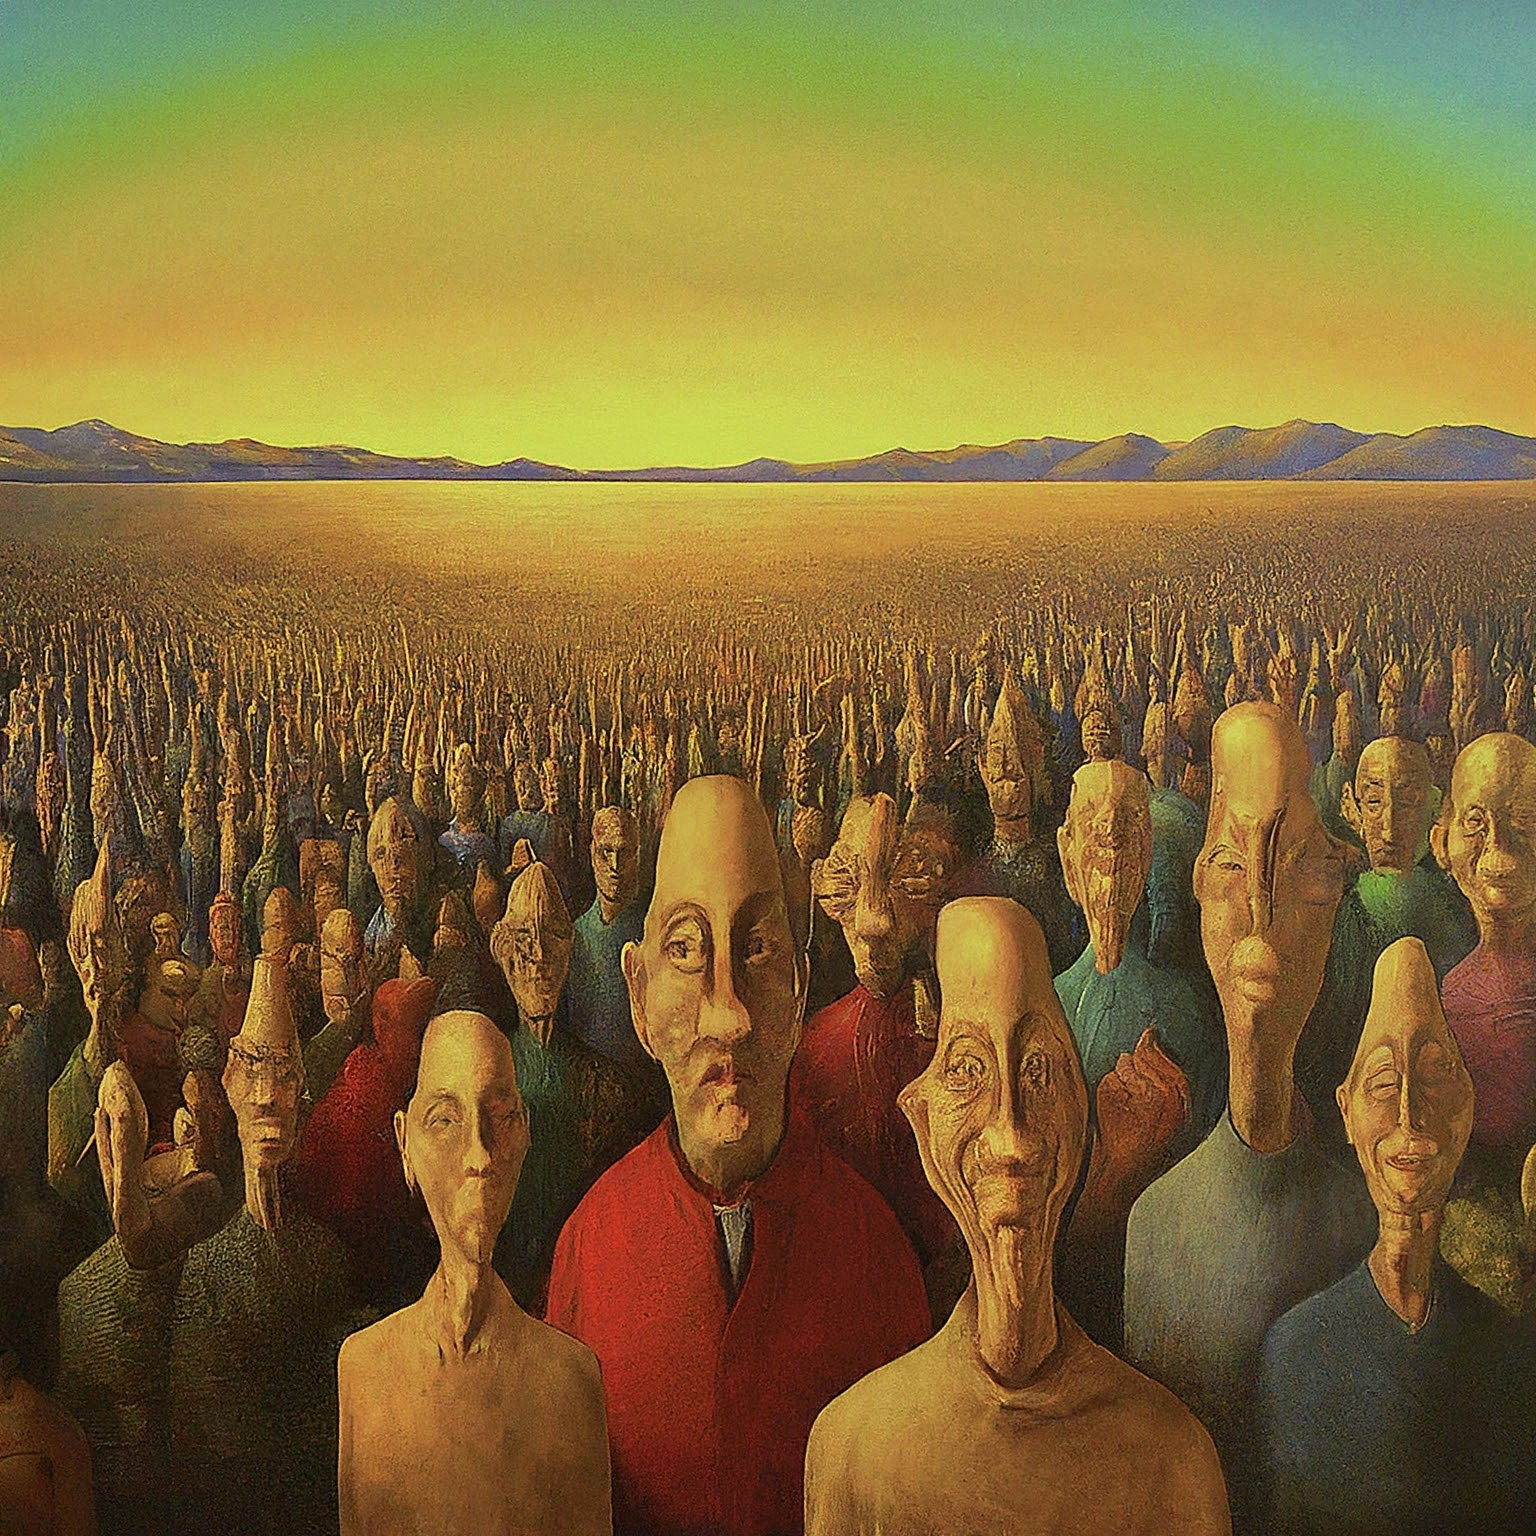
\includegraphics[height=\paperheight,width=\paperwidth]{FIGS/population-models-Gemini_Generated_Image_r55bcer55bcer55b.jpeg}
    };
    \node[anchor=north east,
    inner sep=5pt,
    opacity=0.9] at (current page.north east)
    {
        
\includegraphics[width=0.2\textwidth]{FIGS/UM-logo-horizontal-CMYK.png}
    };
    \node[anchor=south, 
    align=justify, 
    text=black, 
    text width=1.1\textwidth,
    font=\footnotesize]  (land_acknowledgement)
    at (current page.south) 
    {The University of Manitoba campuses are located on original lands of Anishinaabeg, Ininew, Anisininew, Dakota and Dene peoples, and on the National Homeland of the Red River Métis.\\
    We respect the Treaties that were made on these territories, we acknowledge the harms and mistakes of the past, and we dedicate ourselves to move forward in partnership with Indigenous communities in a spirit of Reconciliation and collaboration.};  
    \node[align=center, anchor=south,
    above=0.5cm of land_acknowledgement,
    text=black,
    font=\bfseries] {Fall 2024};
\end{tikzpicture}
  \setbeamercolor{title}{fg=subsub_header_section}
  \setbeamercolor{author}{fg=subsub_header_section} 
  \setbeamerfont{title}{size=\Large,series=\bfseries}
  \setbeamerfont{author}{size=\Large,series=\bfseries}
  \setbeamerfont{date}{series=\bfseries}
	\titlepage
\end{frame}
\addtocounter{page}{-1}


%%%%%%%%%%%%%%%%%%%%%%%%%%%%%%%%%
%%%%%%%%%%%%%%%%%%%%%%%%%%%%%%%%%
%%%%%%%%%%%%%%%%%%%%%%%%%%%%%%%%%
%%%%%%%%%%%%%%%%%%%%%%%%%%%%%%%%%
% The outline page
\begin{frame}[noframenumbering,plain]
  \begin{tikzpicture}[remember picture,overlay]
    \node[above right,inner sep=0pt,opacity=0.2] at (current page.south west)
    {
        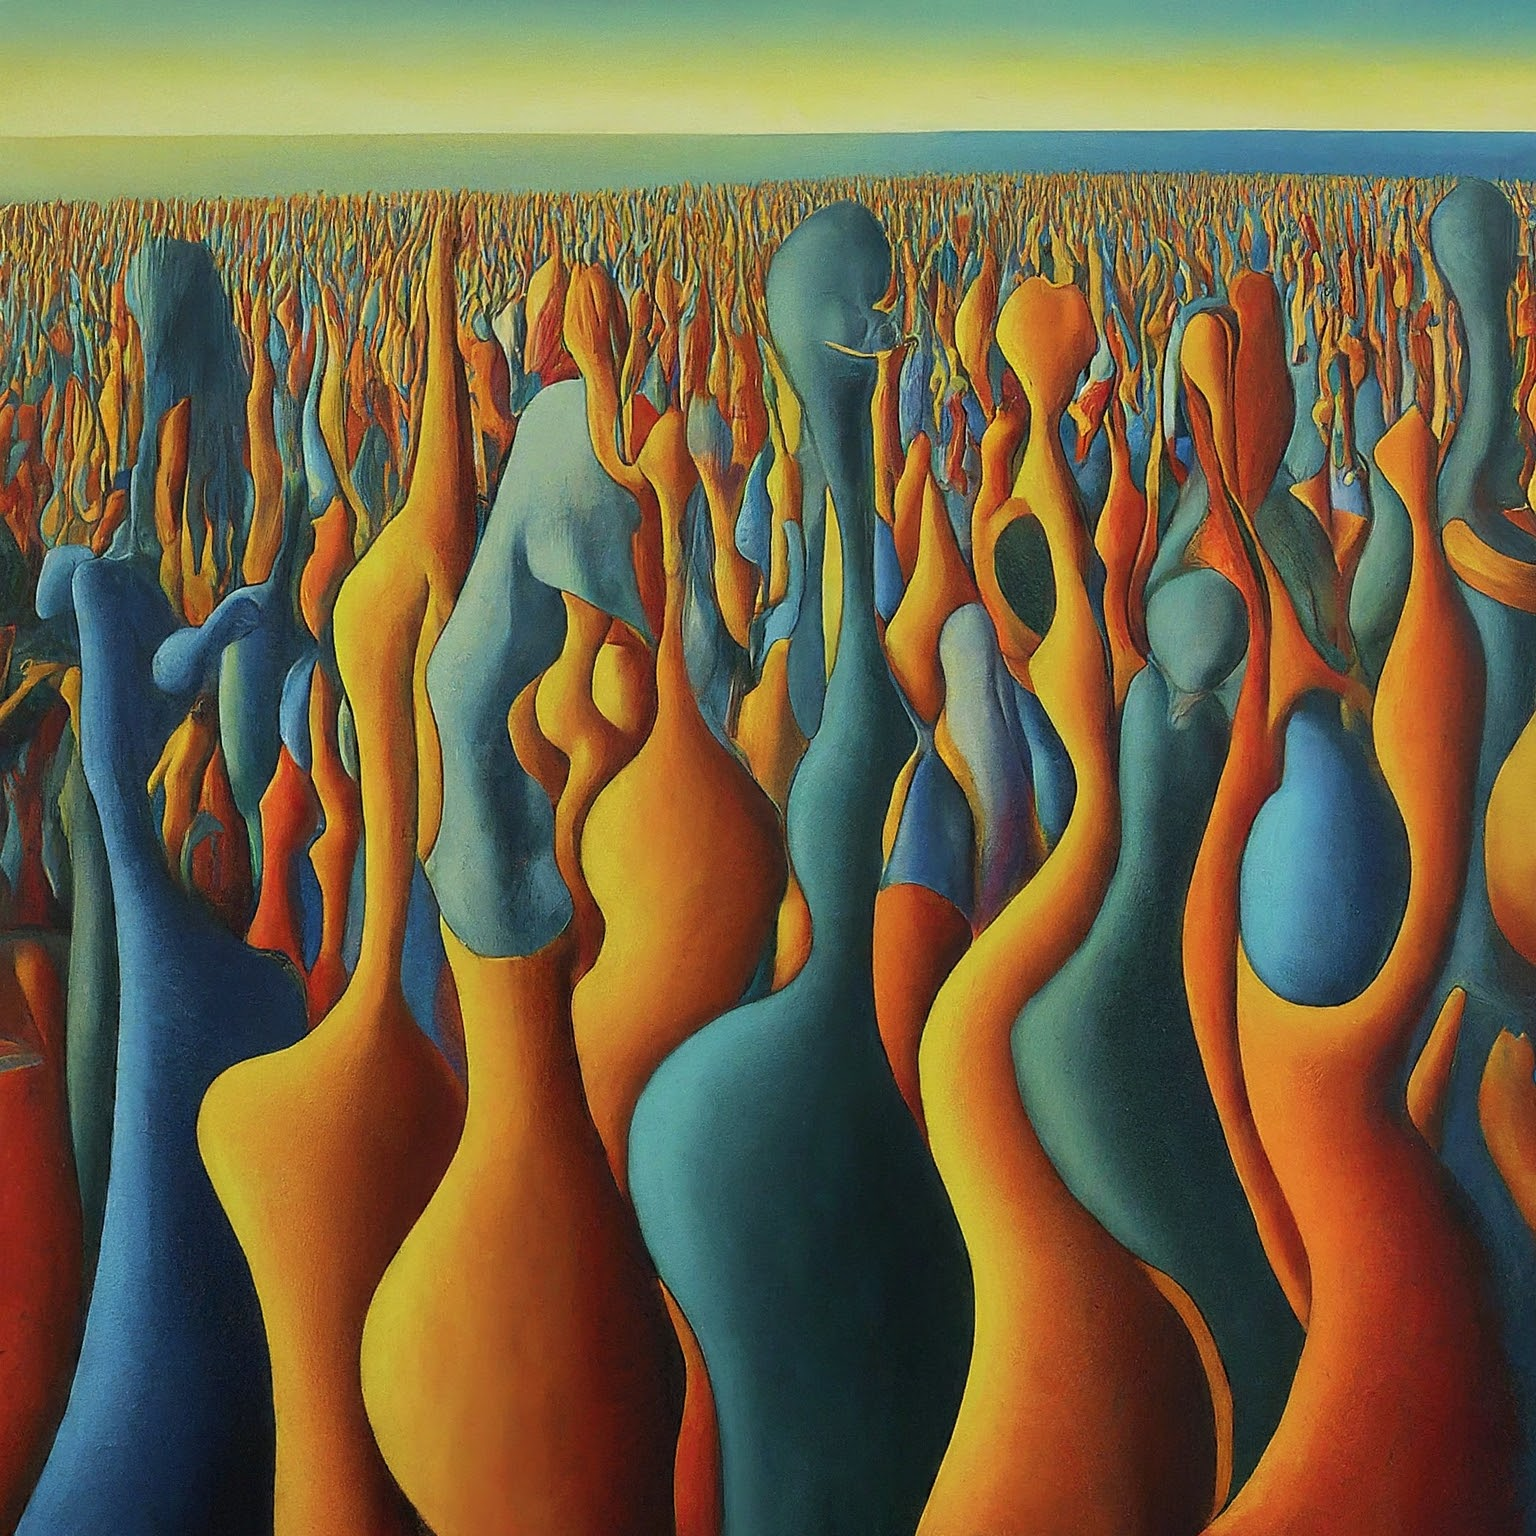
\includegraphics[height=\paperheight,width=\paperwidth]{FIGS/population-models-Gemini_Generated_Image_r55bccr55bccr55b.jpeg}
    };
  \end{tikzpicture}
  \setbeamercolor{section in toc}{fg=subsub_header_section}
  \setbeamerfont{section in toc}{size=\Large,series=\bfseries}
  \frametitle{\textcolor{blue}{\LARGE\bfseries Outline}}
  \tableofcontents[hideallsubsections]
\end{frame}
\addtocounter{page}{-1}



%%%%%%%%%%%%%%%%%%%
%%%%%%%%%%%%%%%%%%%
%%%%%%%%%%%%%%%%%%%
%%%%%%%%%%%%%%%%%%%
\section{Markov chains}
\frame[plain]{\tableofcontents[current]}

\frame{
We conduct an experiment with a set of $r$ outcomes,
\[
S=\{S_1,\dots, S_r\}.
\]
\vskip0.4cm
The experiment is repeated $n$ times (with $n$ large, potentially infinite). 
\vskip0.4cm
The system has \underline{no memory}: the next state depends only on the present state. 
\vskip0.4cm
The probability of $S_j$ occurring on the next step, given that $S_i$ occurred on the last step, is
\[
p_{ij}=p(S_j|S_i).
\]
}

\frame{
Suppose that $S_i$ is the current state, then one of $S_1, \ldots,S_r$ must be the next state; therefore,
\[
p_{i1}+p_{i2}+\cdots+p_{ir}=1, \quad 1\leq i\leq r.
\]
(Note that some of the $p_{ij}$ can be zero, all that is needed is that $\sum_{j=1}^r p_{ij}=1$ for all $i$.)
}

\frame{\frametitle{Markov chain}
\begin{definition}
An experiment with finite number of possible outcomes $S_1,\ldots,S_r$ is repeated. The sequence of outcomes is a \emph{Markov chain} if there is a set of $r^2$ numbers $\{p_{ij}\}$ such that the conditional probability of outcome $S_j$ on any experiment given outcome $S_i$ on the previous experiment is $p_{ij}$, i.e., for $1\leq i,j\leq r$, $n=1,\ldots$,
\[
p_{ij}=\mathsf{Pr}(S_j\textrm{ on experiment }n+1|S_i\textrm{ on experiment }n).
\]
The outcomes $S_1,\ldots,S_r$ are the \emph{states}, and the $p_{ij}$ are the \emph{transition probabilities}. The matrix $P=[p_{ij}]$ is the \emph{transition matrix}.
\end{definition}
}

\frame{\frametitle{Transition matrix}
The matrix 
\[
P=
\begin{pmatrix}
p_{11} & p_{12} & \cdots & p_{1r} \\
p_{21} & p_{22} & \cdots & p_{2r} \\
&&& \\
p_{r1} & p_{r2} & \cdots & p_{rr}
\end{pmatrix}
\]
has
\begin{itemize}
\item nonnegative entries, $p_{ij}\geq 0$
\item entries less than 1, $p_{ij}\leq 1$
\item row sum 1, which we write
\[
\sum_{j=1}^r p_{ij}=1,\quad i=1,\ldots,r
\]
or, using the notation $\nbOne^T=(1,\ldots,1)$,
\[
P\nbOne=\nbOne
\]
\end{itemize}
}


\section{A simple genetic model}
\frame[plain]{\tableofcontents[current]}

\frame{\frametitle{Simple Mendelian inheritance}
A certain trait is determined by a specific pair of genes, each of which may be two types, say $G$ and $g$. 
\vskip0.4cm
One individual may have:
\begin{itemize}
\item $GG$ combination (\emph{dominant})
\item $Gg$ or $gG$, considered equivalent genetically (\emph{hybrid})
\item $gg$ combination (\emph{recessive})
\end{itemize}
\vskip0.4cm
In sexual reproduction, offspring inherit one gene of the pair from each parent. 
}

\frame{\frametitle{Basic assumption of Mendelian genetics}
Genes inherited from each parent are selected at random, independently of each other.
This determines probability
of occurrence of each type of offspring. The offspring
\begin{itemize}
\item of two $GG$ parents must be $GG$, 
\item of two $gg$ parents must be $gg$,
\item of one $GG$ and one $gg$ parent must be $Gg$,
\item other cases must be examined in more detail.
\end{itemize}
}

\frame{\frametitle{$GG$ and $Gg$ parents}
\begin{center}
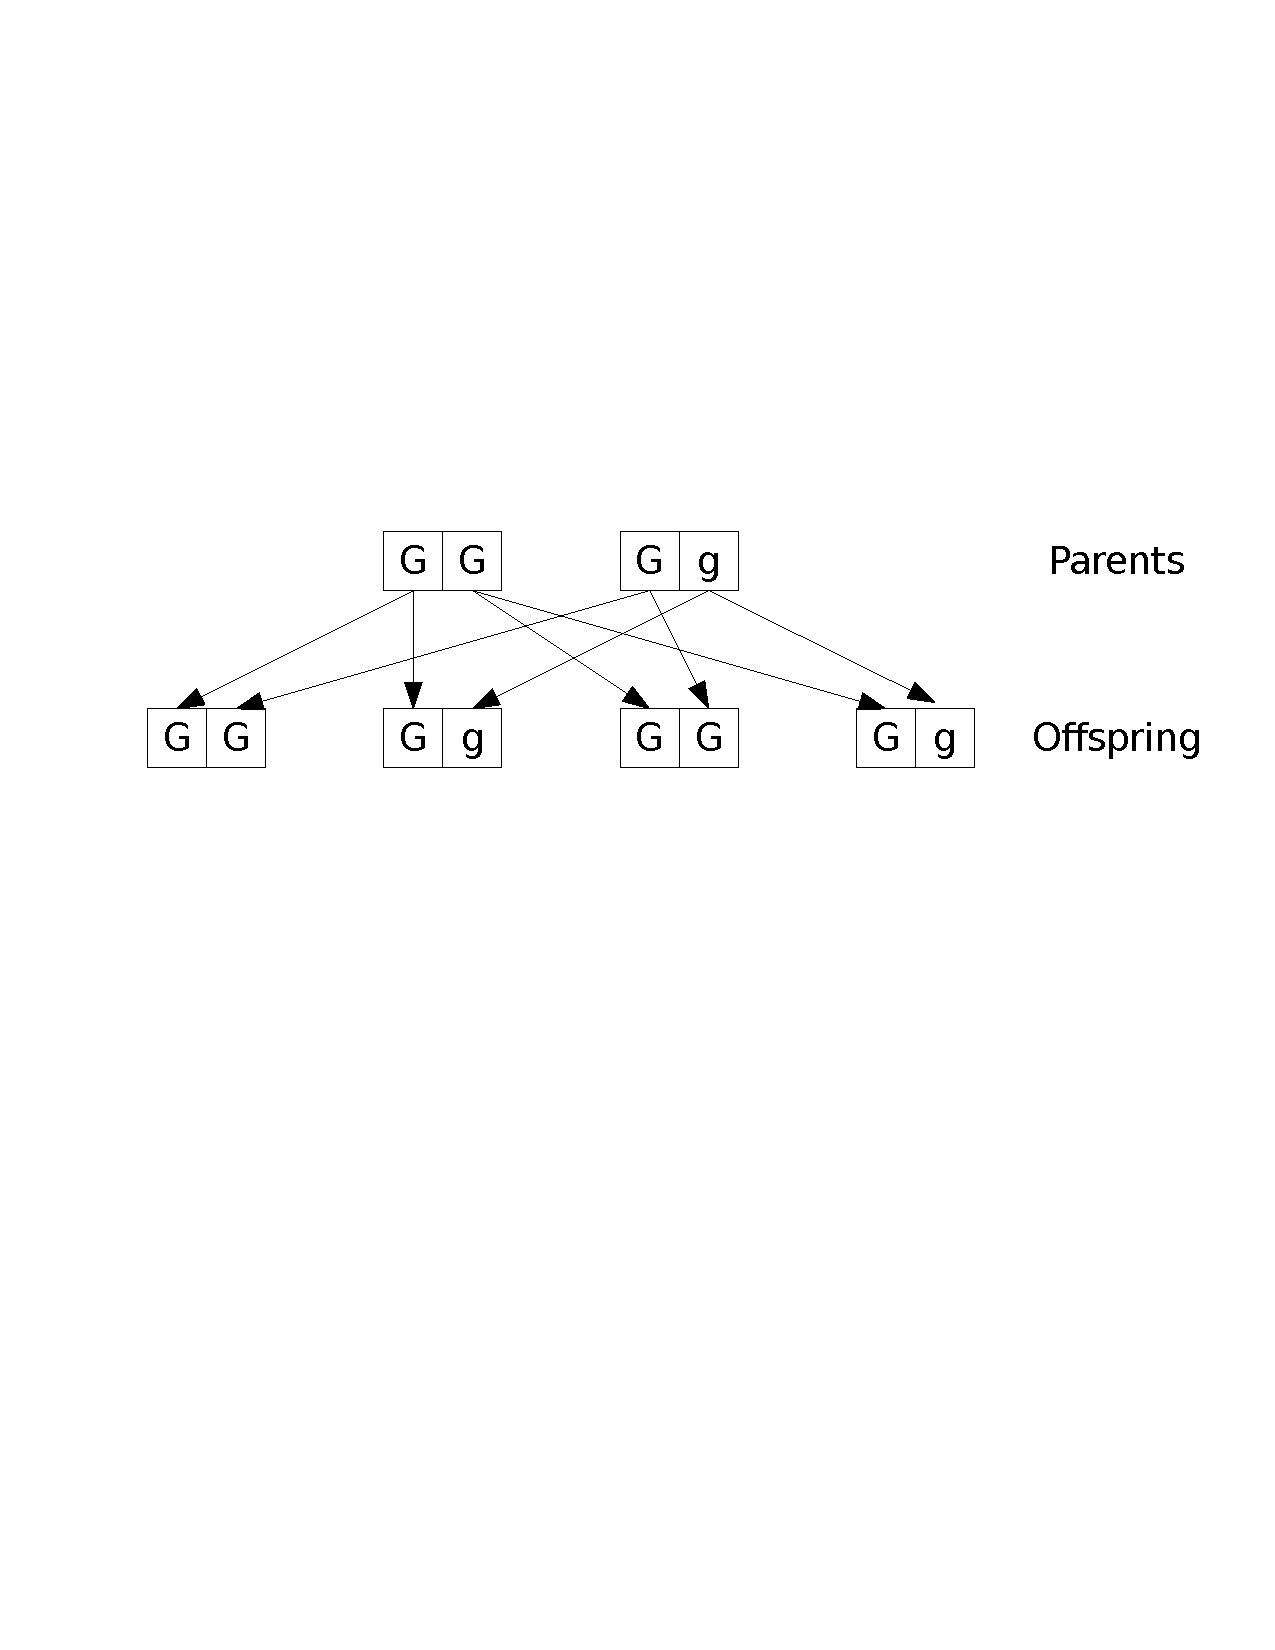
\includegraphics[width=0.9\textwidth]{FIGS/dominant_hybrid}
\end{center}
\vskip0.3cm
Offspring has probability
\begin{itemize}
\item $\dfrac 12$ of being $GG$
\item $\dfrac 12$ of being $Gg$
\end{itemize}
}


\frame{\frametitle{$Gg$ and $Gg$ parents}
\begin{center}
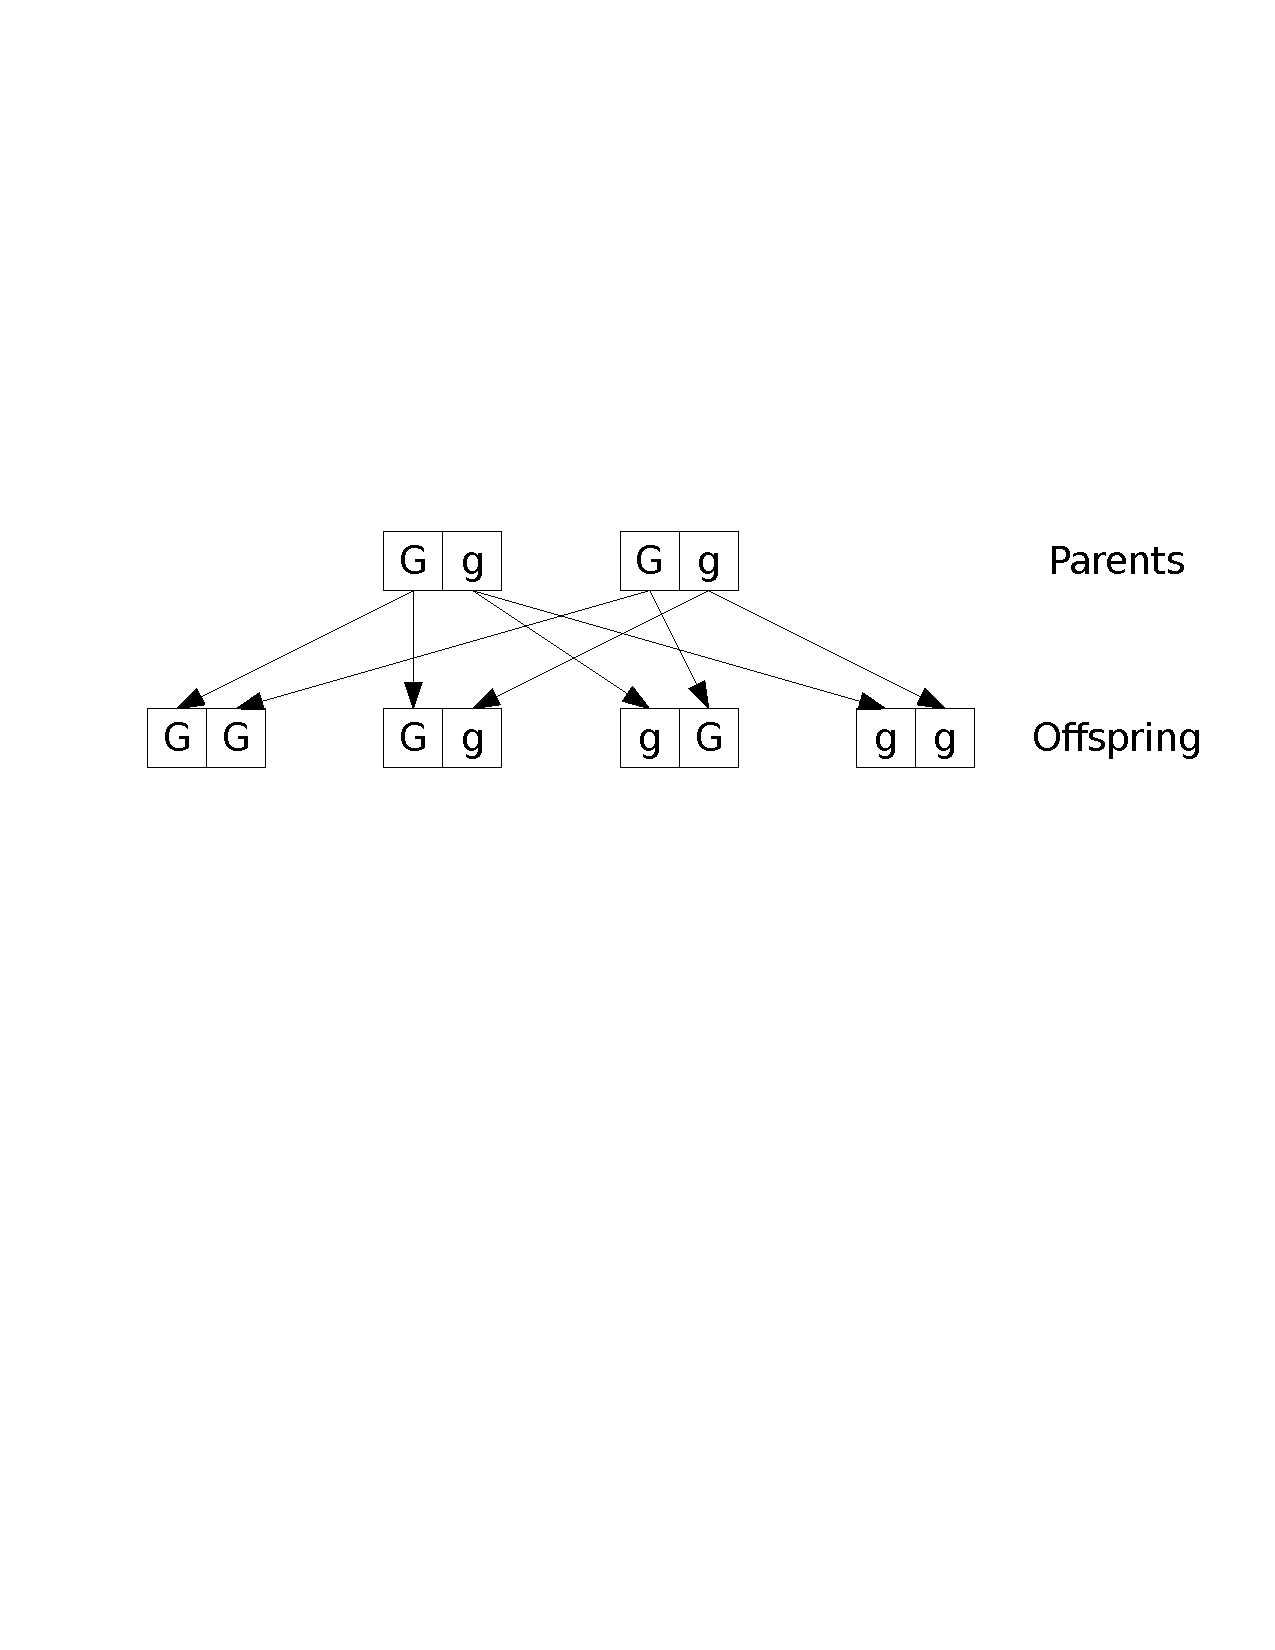
\includegraphics[width=0.9\textwidth]{FIGS/hybrid_hybrid}
\end{center}
\vskip0.3cm
Offspring has probability
\begin{itemize}
\item $\dfrac 14$ of being $GG$
\item $\dfrac 12$ of being $Gg$
\item $\dfrac 14$ of being $gg$
\end{itemize}
}


\frame{\frametitle{$gg$ and $Gg$ parents}
\begin{center}
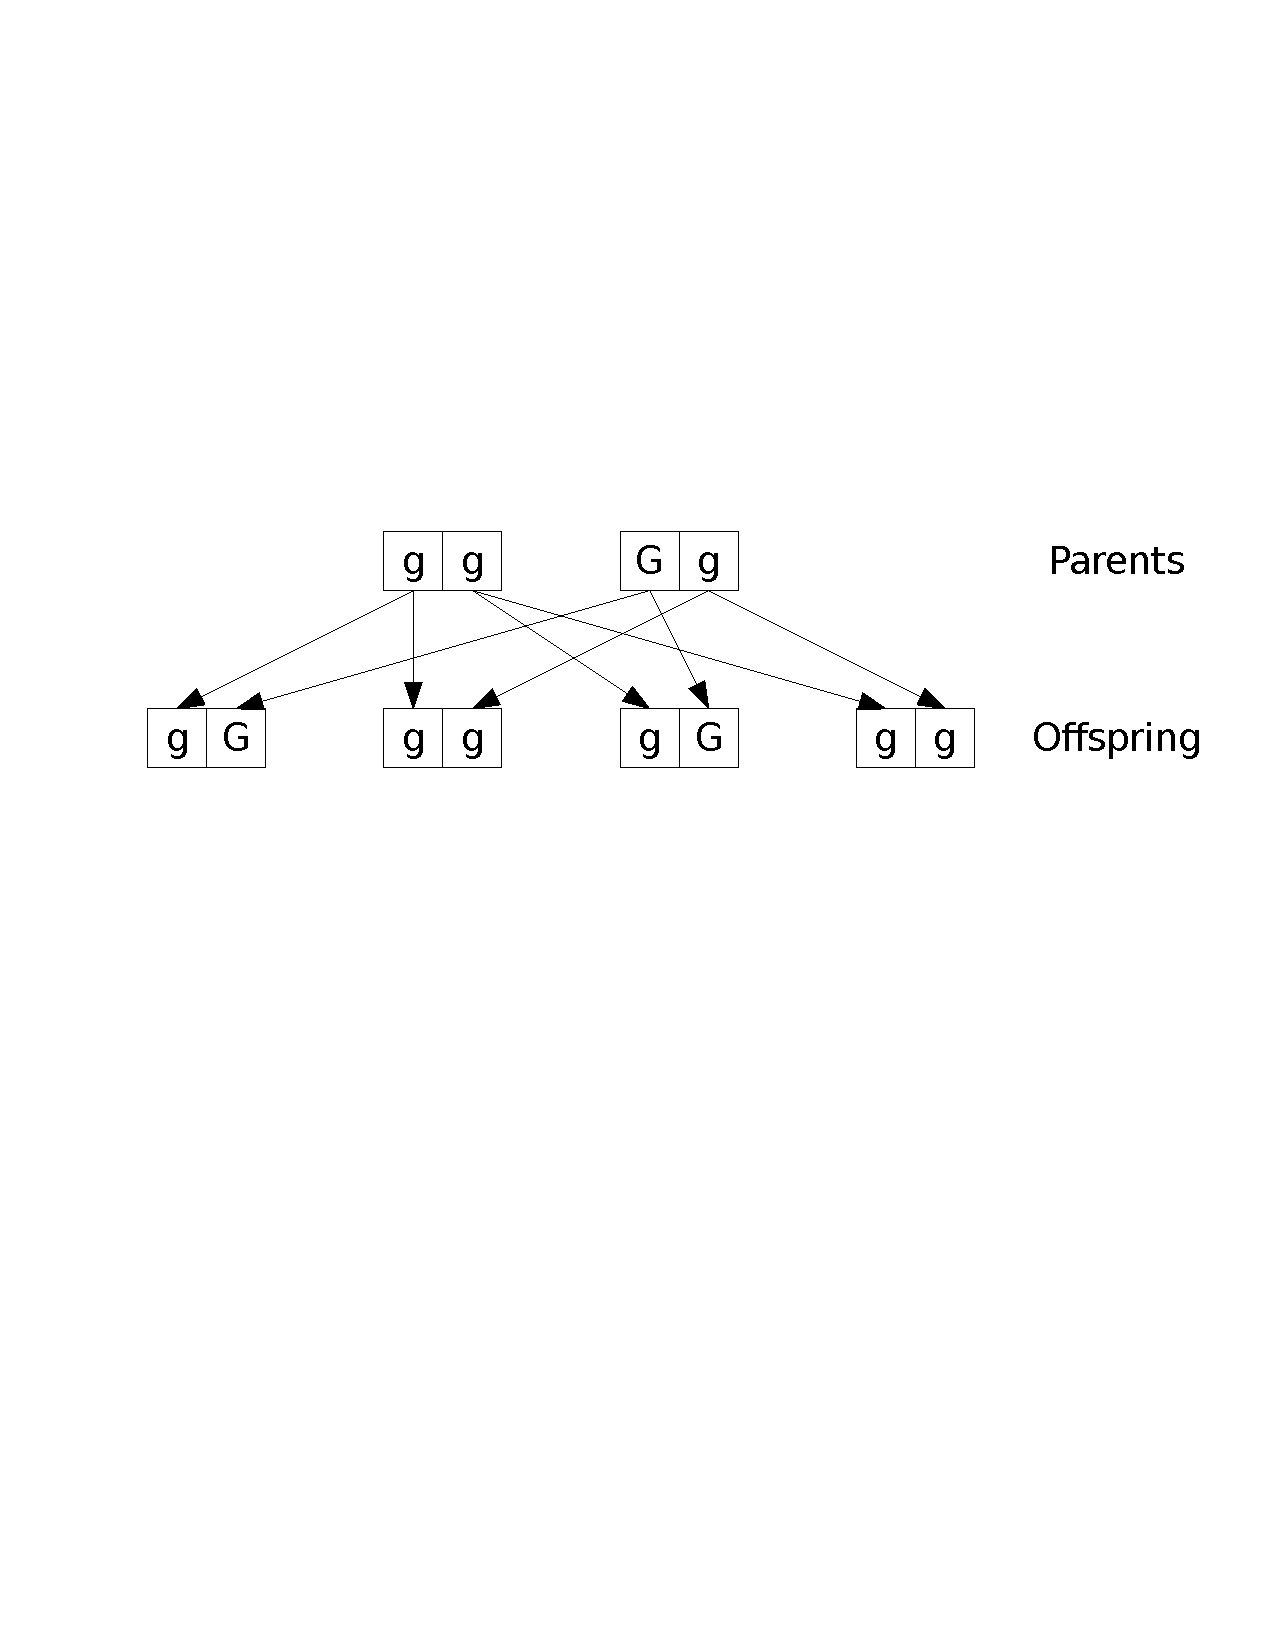
\includegraphics[width=0.9\textwidth]{FIGS/recessive_hybrid}
\end{center}
\vskip0.3cm
Offspring has probability
\begin{itemize}
\item $\dfrac 12$ of being $Gg$
\item $\dfrac 12$ of being $gg$
\end{itemize}
}


\section{Repetition of the process}
\frame[plain]{\tableofcontents[current]}



\frame{\frametitle{General case}
Let $p_i(n)$ be the probability that the state $S_i$ will occur on the $n^{th}$ repetition of the experiment, $1\leq i\leq r$. 
\vskip0.5cm
Since one the states $S_i$ must occur on the $n^{th}$ repetition,
\[
p_1(n)+p_2(n)+\cdots+p_r(n)=1.
\]
}

\frame{
Let $p_i(n+1)$ be the probability that state $S_i$, $1\leq i\leq r$, occurs on $(n+1)^{th}$ repetition of the experiment. 
\vskip0.2cm
There are $r$ ways to be in state $S_i$ at step $n+1$:
\begin{enumerate}
\item Step $n$ is $S_1$. Probability of getting $S_1$ on $n^{th}$ step is $p_1(n)$, and probability of having $S_i$ after $S_1$ is $p_{1i}$. Therefore, by multiplication principle, $P(S_i|S_1)=p_{1i}p_1(n)$. 
\item We get $S_2$ on step $n$ and $S_i$ on step $(n+1)$. Then $P(S_i|S_2)=p_{2i}p_2(n)$. 
\item[..]
\item[r.] Probability of occurrence of $S_i$ at step $n+1$ if $S_r$ at step $n$ is $P(S_i|S_r)=p_{ri}p_r(n)$.
\end{enumerate}
Therefore, $p_i(n+1)$ is sum of all these,
\begin{align*}
p_i(n+1) &= P(S_i|S_1)+\cdots+P(S_i|S_r) \\
&= p_{1i}p_1(n)+\cdots+p_{ri}p_r(n)
\end{align*}
}

\frame{
Therefore,
\begin{equation}\label{eq:chain1}
\begin{aligned}
p_1(n+1) &= p_{11}p_1(n)+p_{21}p_2(n)+\dots+p_{r1}p_r(n) \\
& \vdots\\
p_k(n+1) &= p_{1k}p_1(n)+p_{2k}p_2(n)+\dots+p_{rk}p_r(n) \\
& \vdots\\
p_r(n+1) &= p_{1r}p_1(n)+p_{2r}p_2(n)+\dots+p_{rr}p_r(n)
\end{aligned}
\end{equation}
}

\frame{
In matrix form
\begin{equation}
p(n+1)=p(n)P, \quad n=1,2,3,\dots
\end{equation}
where $p(n)=(p_1(n),p_{2}(n),\dots , p_r(n))$ is a (row) probability vector and $P=(p_{ij})$ is a $r\times r$ \emph{transition matrix},
\[
P=
\begin{pmatrix}
p_{11} & p_{12} & \cdots & p_{1r} \\
p_{21} & p_{22} & \cdots & p_{2r} \\
&&& \\
p_{r1} & p_{r2} & \cdots & p_{rr}
\end{pmatrix}
\]
}

\frame{
So, what we have is
\begin{multline*}
(p_1(n+1),\ldots,p_r(n+1))= \\
(p_1(n),\ldots,p_r(n))
\begin{pmatrix}
p_{11} & p_{12} & \cdots & p_{1r} \\
p_{21} & p_{22} & \cdots & p_{2r} \\
&&& \\
p_{r1} & p_{r2} & \cdots & p_{rr}
\end{pmatrix}
\end{multline*}
It is easy to check that this gives the same expression as \eqref{eq:chain1}.
}



\frame{\frametitle{For our genetic model..}
Consider a process of continued matings. 
\begin{itemize}
\item Start with an individual of known or unknown
genetic character and mate it with a hybrid. 
\item Assume that there is at least one
offspring; choose one of them at random and mate it with a hybrid.
\item Repeat this process through a number of generations. 
\end{itemize}
The genetic type of the chosen
offspring in successive generations can be represented by a Markov chain, with states $GG$, $Gg$ and $gg$. So there are 3 possibles states $S_1=GG$, $S_2=Gg$ and $S_3=gg$.
}

\frame{
We have
\begin{center}
\begin{tabular}{c|ccc}
$\nearrow$ & GG & Gg & gg \\
\hline
GG & 0.5 & 0.5 & 0 \\
Gg & 0.25 & 0.5 & 0.25 \\
gg & 0 & 0.5 & 0.5
\end{tabular}
\end{center}
The transition probabilities are thus
\[
P=\left (
\begin{array}{ccc}
\frac 12 & \frac 12 & 0 \\
\frac 14 & \frac 12 & \frac 14 \\
0 & \frac 12 & \frac 12
\end{array}\right)
\]
}

\frame{\frametitle{Stochastic matrices}
\begin{definition}[Stochastic matrix]
The nonnegative $r\times r$ matrix $M$ is \emph{stochastic} if $\sum_{j=1}^ra_{ij}=1$ for all $i=1,2,\dots, r$.
\end{definition}
\begin{theorem}
Let $M$ be a stochastic matrix $M$. Then all eigenvalues $\lambda$ of $M$ are such that $|\lambda|\leq 1$. 
Furthermore, $\lambda =1$ is an eigenvalue of $M$.
\end{theorem}
\vskip0.4cm
To see that $1$ is an eigenvalue, write the definition of a stochastic matrix, i.e., $M$ has row sums 1. In vector form, $M\nbOne=\nbOne$. Now remember that $\lambda$ is an eigenvalue of $M$, with associated eigenvector $v$, iff $Mv=\lambda v$. So, in the expression $M\nbOne=\nbOne$, we read an eigenvector, $\nbOne$, and an eigenvalue, $1$.
}

\frame{\frametitle{Long ``time'' behavior}
Let $p(0)$ be the initial distribution (row) vector. Then
\begin{align*}
p(1) &= p(0)P \\
p(2) &= p(1)P\\
&= (p(0)P)P \\
&= p(0)P^2
\end{align*}
Iterating, we get that for any $n$,
\[
p(n)=p(0)P^n
\]
Therefore, 
\[
\lim_{n\rightarrow +\infty}p(n)=\lim_{n\rightarrow +\infty}p(0)P^n=p(0)\lim_{n\rightarrow +\infty}P^n
\]
}

\frame{\frametitle{Additional properties of stochastic matrices}
\begin{theorem}
If $M,N$ are stochastic matrices, then $MN$ is a stochastic matrix.
\end{theorem}
\begin{theorem}
If $M$ is a stochastic matrix, then for any $k\in\IN$, $M^k$ is a stochastic matrix.
\end{theorem}
}

\section{Regular Markov chains}
\frame[plain]{\tableofcontents[current]}


\frame{\frametitle{Regular Markov chain}
\begin{definition}[Regular Markov chain]
A regular Markov chain is one in which $P^k$ is positive for some integer $k>0$, i.e., $P^k$ has only positive entries, no zero entries.
\end{definition}
\begin{definition}
A nonnegative matrix $M$ is primitive if, and only if, there is an integer $k>0$ such that $M^k$ is positive.
\end{definition}
\begin{theorem}
A Markov chain is regular if, and only if, the transition matrix $P$ is primitive.
\end{theorem}
}

\frame{\frametitle{Important result for regular Markov chains}
\begin{theorem}
If $P$ is the transition matrix of a regular Markov chain, then
\begin{enumerate}
\item the powers $P^n$ approach a stochastic matrix $W$,
\item each row of $W$ is the same (row) vector $w=(w_1,\ldots,w_r)$,
\item the components of $w$ are positive.
\end{enumerate}
\end{theorem}
So if the Markov chain is regular,
\[
\lim_{n\rightarrow +\infty}p(n)=p(0)\lim_{n\rightarrow +\infty}P^n
=p(0)W
\]
}


\frame{\frametitle{Left and right eigenvectors}
Let $M$ be an $r\times r$ matrix, $u,v$ be two column vectors, $\lambda\in\IR$. Then, if  
\[
Mu=\lambda u,
\]
$u$ is the (right) eigenvector corresponding to $\lambda$, and if
\[
v^TM=\lambda v^T
\]
then $v$ is the left eigenvector corresponding to $\lambda$. Note that to a given eigenvalue there corresponds one left and one right eigenvector.
}

\frame{
The vector $w$ is in fact the left eigenvector corresponding to the eigenvalue 1 of $P$. (We already know that the (right) eigenvector corresponding to 1 is $\nbOne$.)
\vskip0.5cm
To see this, remark that, if $p(n)$ converges, then $p(n+1)=p(n)P$, so $w$ is a fixed point of the system. We thus write
\[
wP=w
\]
and solve for $w$, which amounts to finding $w$ as the left eigenvector corresponding to the eigenvalue 1.
\vskip0.5cm
Alternatively, we can find $w$ as the (right) eigenvector associated to the eigenvalue 1 for the transpose of $P$,
\[
P^Tw^T=w^T
\]
}

\frame{
Now remember that when you compute an eigenvector, you get a result that is the eigenvector, to a multiple.
\vskip1cm
So the expression you obtain for $w$ might have to be normalized (you want a probability vector). Once you obtain $w$, check that the norm $\|w\|$ defined by
\[
\|w\|=w_1+\cdots+w_r
\]
is equal to one. If not, use
\[
\frac{w}{\|w\|}
\]
}

\frame{\frametitle{Back to genetics..}
The Markov chain is here regular. Indeed, take the matrix $P$,
\[
P=\left (
\begin{array}{ccc}
\frac 12 & \frac 12 & 0 \\
\frac 14 & \frac 12 & \frac 14 \\
0 & \frac 12 & \frac 12
\end{array}\right)
\]
and compute $P^2$:
\[
P^2=\left (
\begin{array}{ccc}
\frac 38 & \frac 12 & \frac 18 \\
\frac 14 & \frac 12 & \frac 14 \\
\frac 18 & \frac 12 & \frac 38
\end{array}\right)
\]
As all entries are positive, $P$ is primitive and the Markov chain is regular.
}

\frame{
Another way to check regularity:
\begin{theorem}
A matrix $M$ is primitive if the associated connection graph is strongly connected, i.e., that there is a path between any pair $(i,j)$ of states, and that there is at least one positive entry on the diagonal of $M$.
\end{theorem}
This is checked directly on the transition graph
\begin{center}
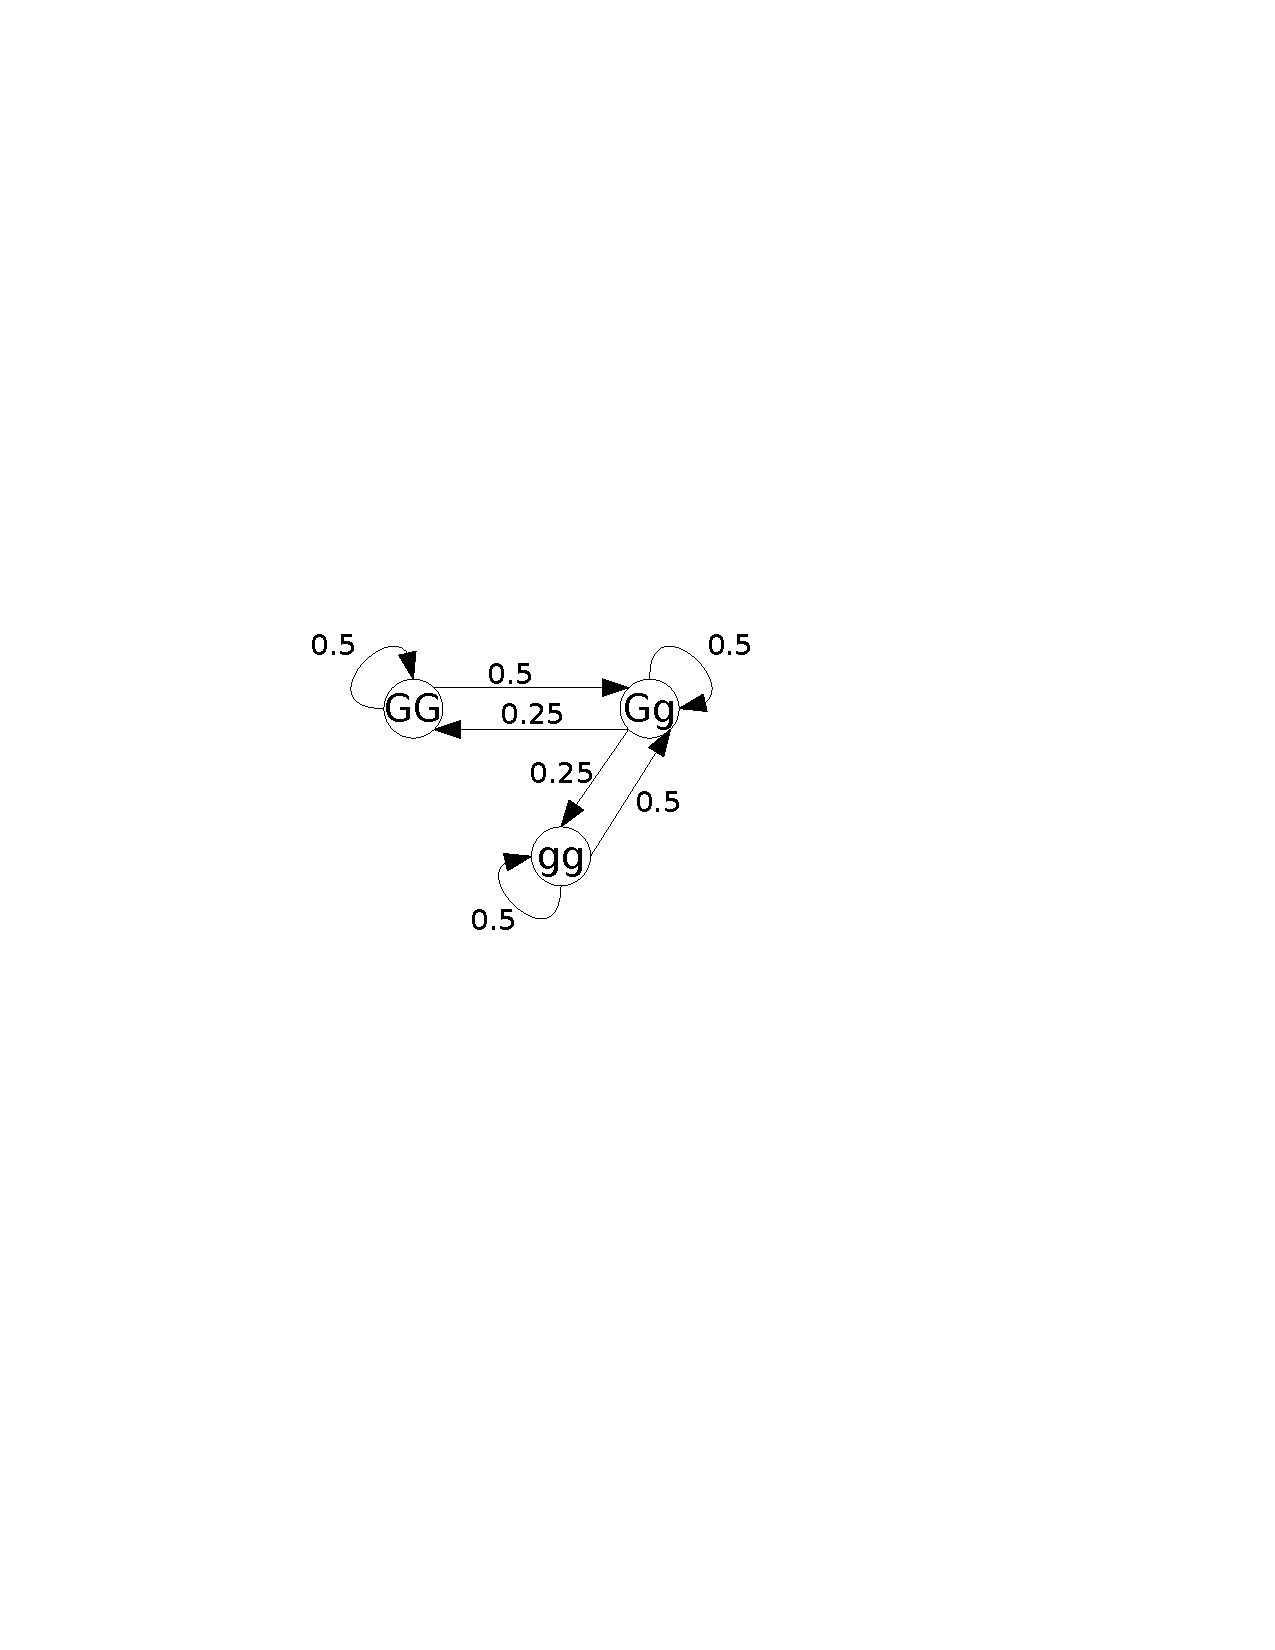
\includegraphics[width=0.6\textwidth]{FIGS/graphe_hybride}
\end{center}
}

\frame{
Compute the left eigenvector associated to 1 by solving
\[
(w_1,w_2,w_3)
\left (
\begin{array}{ccc}
\frac 12 & \frac 12 & 0 \\
\frac 14 & \frac 12 & \frac 14 \\
0 & \frac 12 & \frac 12
\end{array}\right)=(w_1,w_2,w_3)
\]
\begin{subequations}
\begin{align}
\frac 12 w_1+\frac 14 w_2 &= w_1 \label{eq:l1} \\
\frac 12 w_1+\frac 12 w_2+\frac 12 w_3 &= w_2 \label{eq:l2} \\
\frac 14 w_2+\frac 12 w_3 &= w_3 \label{eq:l3} 
\end{align}
\end{subequations}
From \eqref{eq:l1}, $w_1=w_2/2$, and from \eqref{eq:l3}, $w_3=w_2/2$. Substituting these values into \eqref{eq:l2},
\[
\frac 14 w_2+\frac 12 w_2 +\frac 14 w_2=w_2,
\]
that is, $w_2=w_2$, i.e., $w_2$ can take any value. So $w=(\frac 14,\frac 12,\frac 14)$.
}

\section{Absorbing Markov chains}
\frame[plain]{\tableofcontents[current]}


\frame{\frametitle{Mating with a $GG$ individual}
Suppose now that we conduct the same experiment, but mate each new generation with a $GG$ individual instead of a $Gg$ individual. Transition table is
\begin{center}
\begin{tabular}{c|ccc}
$\nearrow$ & GG & Gg & gg \\
\hline
GG & 1 & 0 & 0 \\
Gg & 0.5 & 0.5 & 0 \\
gg & 0 & 1 & 0
\end{tabular}
\end{center}
The transition probabilities are thus
\[
P=\left (
\begin{array}{ccc}
1 & 0 & 0 \\
\frac 12 & \frac 12 & 0 \\
0 & 1 & 0
\end{array}\right)
\]
}

\frame{\frametitle{New transition graph}
\begin{center}
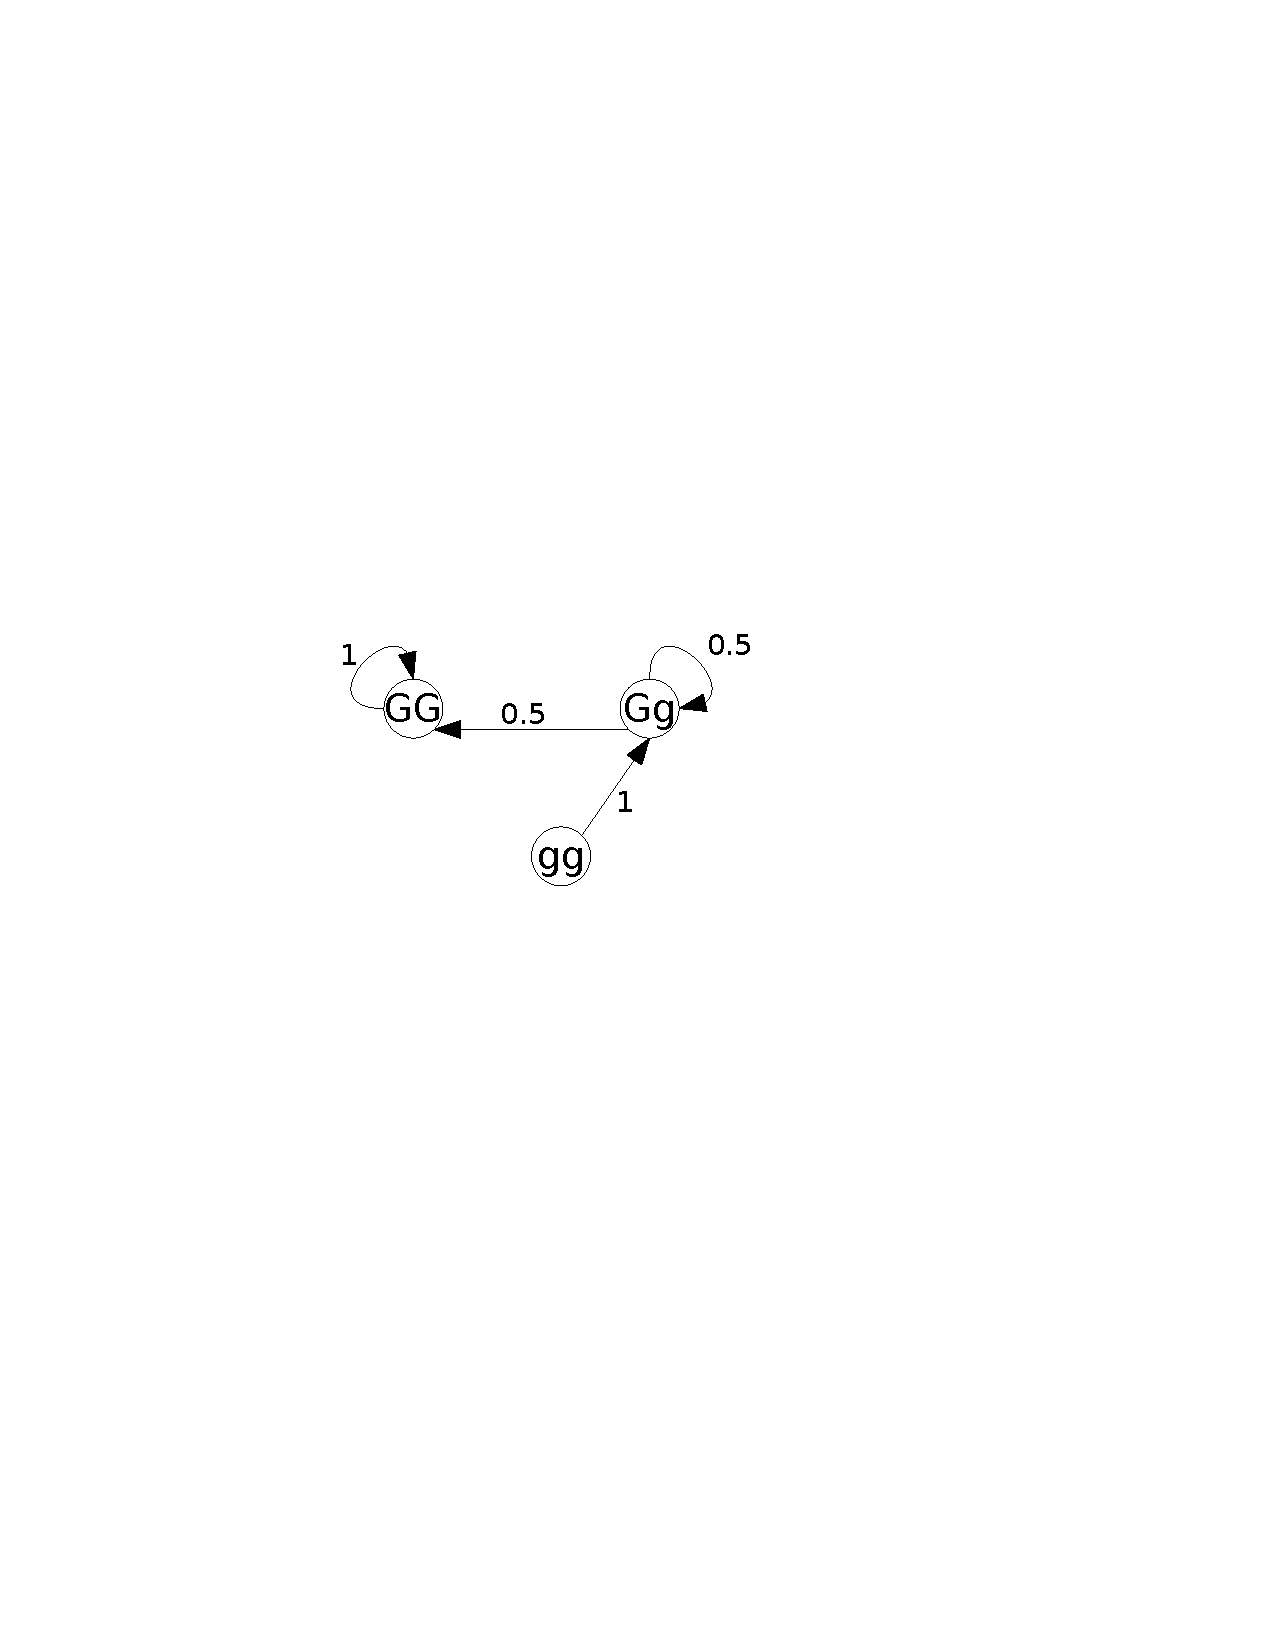
\includegraphics[width=0.8\textwidth]{FIGS/graphe_dominant}
\end{center}
Clearly: 
\begin{itemize}
\item we leave $gg$ after one iteration, and can never return,
\item as soon as we leave $Gg$, we can never return,
\item can never leave $GG$ as soon as we get there.
\end{itemize}
}


\frame{\frametitle{Absorbing states, absorbing chains}
\begin{definition}
A state $S_i$ in a Markov chain is \emph{absorbing} if whenever it occurs on the $n^{th}$ generation of the experiment, it then occurs on every subsequent step. In other words, $S_i$ is absorbing if $p_{ii}=1$ and $p_{ij}=0$ for $i\neq j$.
\end{definition}

\begin{definition}
A Markov chain is said to be absorbing if it has at least one absorbing state, and if from every state it is possible to go to an absorbing state.
\end{definition}

In an absorbing Markov chain, a state that is not absorbing is called \emph{transient}.
}


\frame{\frametitle{Some questions on absorbing chains}
Suppose we have a chain like the following:
\begin{center}
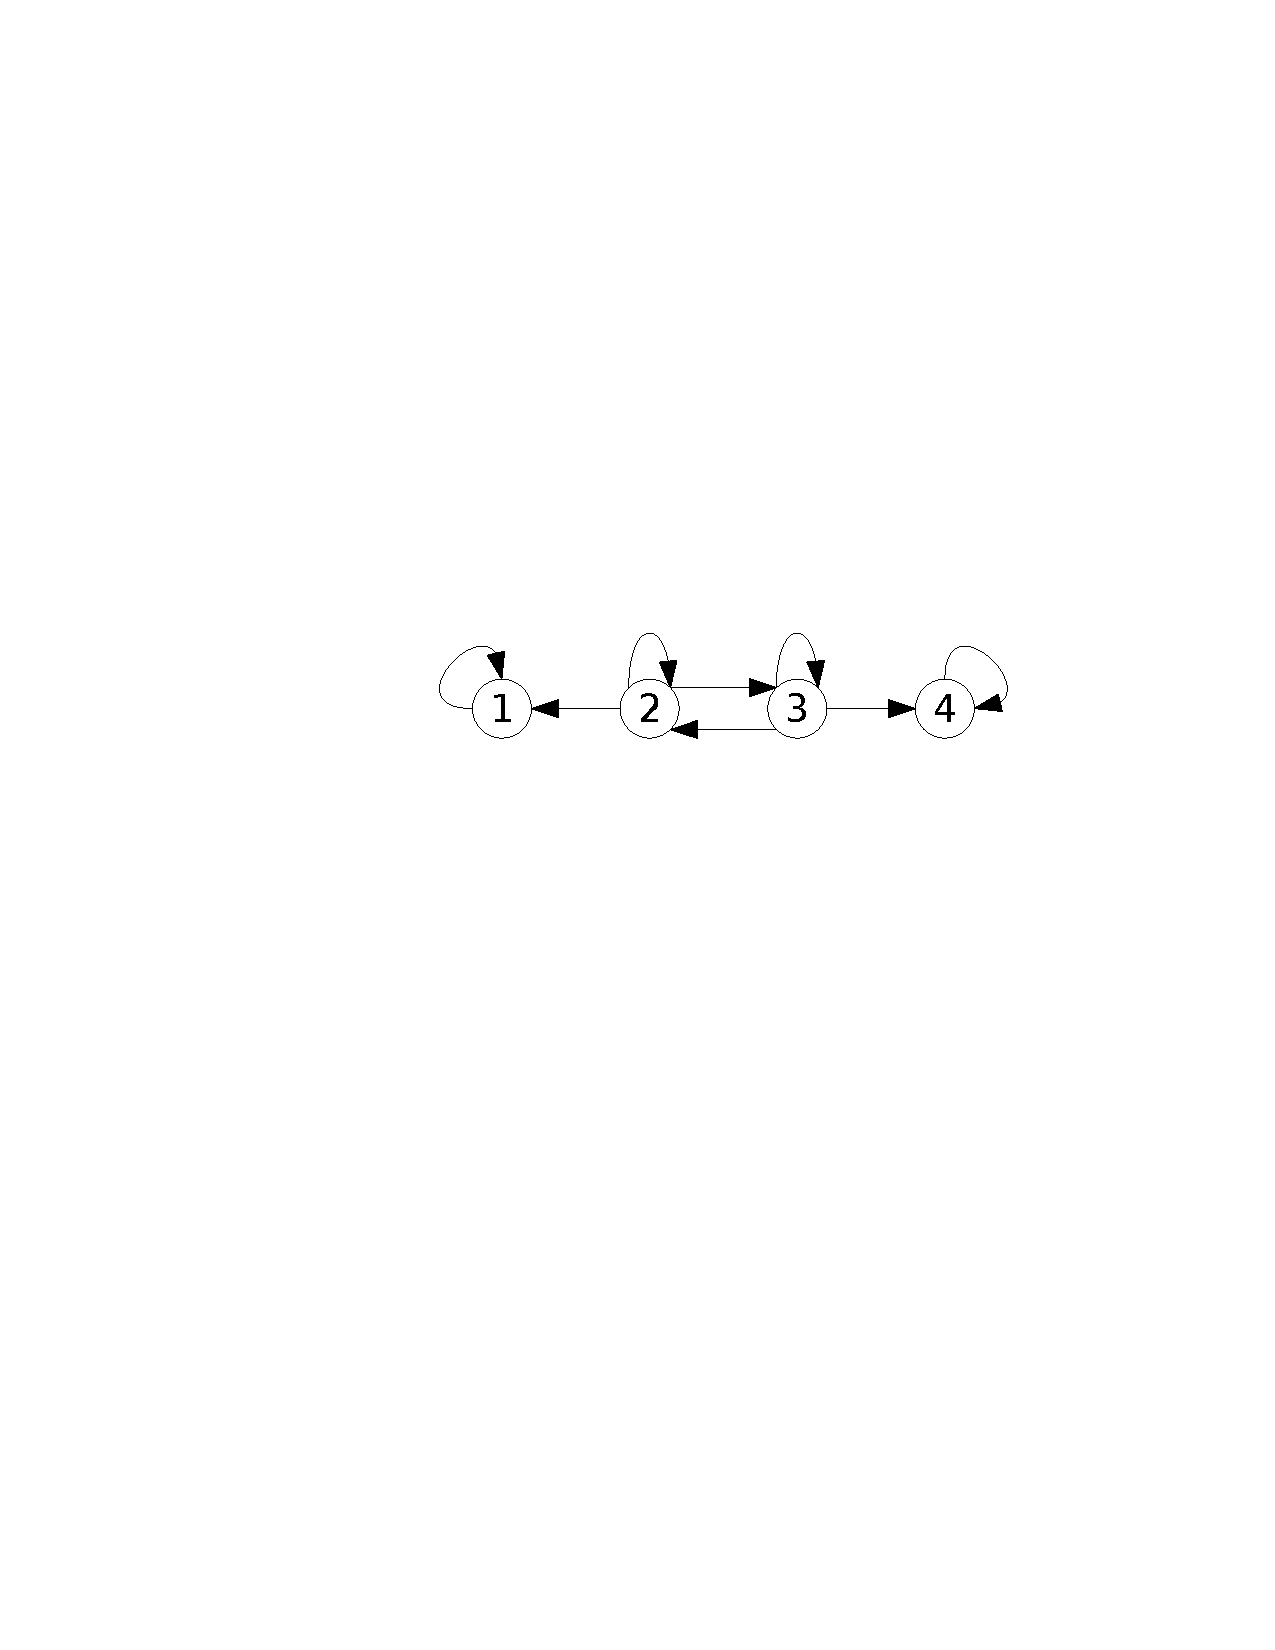
\includegraphics[width=0.8\textwidth]{FIGS/graphe_absorbant}
\end{center}
\begin{enumerate}
\item Does the process eventually reach an absorbing state?
\item Average number of times spent in a transient state, if starting in a transient state?
\item Average number of steps before entering an absorbing state?
\item Probability of being absorbed by a given absorbing state, when there are more than one, when starting in a given transient state?
\end{enumerate}
}

\frame{\frametitle{Reaching an absorbing state}
Answer to question 1:
\begin{theorem}
In an absorbing Markov chain, the probability of reaching an absorbing state is 1.
\end{theorem}
}

\frame{\frametitle{Standard form of the transition matrix}
For an absorbing chain with $k$ absorbing states and $r-k$ transient states, the transition matrix can be written as
\[
P=\begin{pmatrix}
\mathbb{I}_k & \mathbf{0} \\
R & Q
\end{pmatrix}
\]
with following meaning,
\begin{center}
\begin{tabular}{ccc}
& Absorbing states & Transient states \\
Absorbing states & $\mathbb{I}_k$ & $\mathbf{0}$ \\
Transient states & $R$ & $Q$
\end{tabular}
\end{center}
with $\mathbb{I}_k$ the $k\times k$ identity matrix, $\mathbf{0}$ an $k\times(r-k)$ matrix of zeros, $R$ an $(r-k)\times k$ matrix and $Q$ an $(r-k)\times(r-k)$ matrix.
}

\frame{
The matrix $\mathbb{I}_{r-k}-Q$ is invertible. Let
\begin{itemize}
\item $N=(\mathbb{I}_{r-k}-Q)^{-1}$ be the \emph{fundamental matrix} of the Markov chain
\item $T_i$ be the sum of the entries on row $i$ of $N$
\item $B=NR$.
\end{itemize}
\vskip0.5cm
Answers to our remaining questions:
\begin{enumerate}
\setcounter{enumi}{1}
\item $N_{ij}$ is the average number of times the process is in the $j$th transient state if it starts in the $i$th transient state.
\item $T_i$ is the average number of steps before the process enters an absorbing state if it starts in the $i$th transient state.
\item $B_{ij}$ is the probability of eventually entering the $j$th absorbing state if the process starts in the $i$th transient state.
\end{enumerate}
}


\frame{\frametitle{Back to genetics..}
The matrix is already in standard form,
\[
P=\left (
\begin{array}{ccc}
1 & 0 & 0 \\
\frac 12 & \frac 12 & 0 \\
0 & 1 & 0
\end{array}\right)
=\begin{pmatrix}
\mathbb{I}_1 & \mathbf{0} \\
R & Q
\end{pmatrix}
\]
with $\mathbb{I}_1=1$, $\mathbf{0}=(0\;\; 0)$ and
\[
R=\begin{pmatrix}
\frac 12\\ 0
\end{pmatrix}
\qquad
Q=\begin{pmatrix}
\frac 12 & 0\\
1 & 0
\end{pmatrix}
\]
}

\frame{
We have
\[
\mathbb{I}_2-Q=\begin{pmatrix}
1 & 0 \\
0 & 1
\end{pmatrix}
-\begin{pmatrix}
\frac 12 & 0\\
1 & 0
\end{pmatrix}
=\begin{pmatrix}
\frac 12 & 0\\
-1 & 1
\end{pmatrix}
\]
so
\[
N=(\mathbb{I}_2-Q)^{-1}=
2\begin{pmatrix}
1 & 0 \\
1 & \frac 12
\end{pmatrix}=
\begin{pmatrix}
2 & 0 \\
2 & 1
\end{pmatrix}
\]
Then
\[
T=N\nbOne=\begin{pmatrix}
2\\
3
\end{pmatrix}
\]
and
\[
B=NR=
\begin{pmatrix}
2 & 0 \\
2 & 1
\end{pmatrix}
\begin{pmatrix}
\frac 12\\ 0
\end{pmatrix}
=
\begin{pmatrix}
1\\ 1
\end{pmatrix}
\]
}

\section{Random walks}

\frame{\frametitle{The drunk man's walk, 1.0}
\begin{itemize}
\item chain of states $S_1,\ldots,S_p$
\item if in state $S_i$, $i=2,\ldots,p-1$, probability 1/2 of going left (to $S_{i-1}$) and 1/2 of going right (to $S_{i+1}$)
\item if in state $S_1$, probability 1 of going to $S_2$
\item if in state $S_p$, probability 1 of going to $S_{p-1}$
\end{itemize}
\vskip1cm
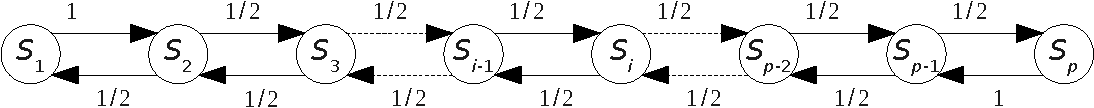
\includegraphics[width=\textwidth]{FIGS/drunk_mans_walk_regular}
}


\frame{\frametitle{The transition matrix for DMW 1.0}
\[
P=\begin{pmatrix}
0 & 1 & 0 & 0 & 0 & \cdots & 0\\
1/2 & 0 & 1/2 & 0 & & & \\
0 & 1/2 & 0 & 1/2 & & & \\
\vdots & & \ddots & \ddots & \ddots & & \vdots \\
& & & & & & \\
& & & & 1/2 & 0 & 1/2 \\
& & & & 0 & 1 & 0
\end{pmatrix}
\]
Clearly a primitive matrix, so this is an regular Markov chain.
}

\frame{
We need to solve $w^TP=w^T$, that is,
\begin{align*}
\frac 12 w_2 &= w_1 \\
w_1 +\frac 12 w_3 &= w_2 \\
\frac 12 w_2+\frac 12 w_4 &= w_3 \\
\frac 12 w_3+\frac 12 w_5 &= w_4 \\
& \vdots \\
\frac 12 w_{p-3}+\frac 12 w_{p-1} &= w_{p-2} \\
\frac 12 w_{p-2}+w_p &= w_{p-1} \\
\frac 12 w_{p-1} &= w_p
\end{align*}
}

\frame{
Express everything in terms of $w_1$:
\begin{align*}
w_2 &= 2w_1 \\
w_1 +\frac 12 w_3 &= w_2 \Leftrightarrow w_3 = 2(w_2-w_1)=2w_1\\
\frac 12 w_2+\frac 12 w_4 &= w_3 \Leftrightarrow w_4=2(w_3-\frac 12 w_2)=2(w_3-w_1)=2w_1\\
\frac 12 w_3+\frac 12 w_5 &= w_4 \Leftrightarrow w_5=2(w_4-\frac 12 w_3)=2(w_4-w_1)=2w_1\\
& \vdots \\
\frac 12 w_{p-3}+\frac 12 w_{p-1} &= w_{p-2} \Leftrightarrow w_{p-1} = 2w_1 \\
\frac 12 w_{p-2}+w_p &= w_{p-1} \Leftrightarrow w_p=w_{p-1}-\frac 12 w_{p-2}=w_1\\
\frac 12 w_{p-1} &= w_p \qquad (\textrm{confirms that }w_p=w_1)
\end{align*}
}

\frame{
So we get
\[
w^T=\left(w_1,2w_1,\ldots,2w_1,w_1\right)
\]
We have
\begin{align*}
\sum_{i=1}^p w_i &= w_1+\left(\sum_{i=2}^{p-1}2w_1\right)+w_1 \\
&= 2w_1+\sum_{i=2}^{p-1}2w_1 \\
&= \sum_{i=1}^{p-1} 2w_1  \\
&= 2w_1\sum_{i=1}^{p-1}1  \\
&= 2w_1(p-1)
\end{align*}
}

\frame{
Since 
\[
\sum_{i=1}^p w_i = 2w_1(p-1)
\]
to get a probability vector, we need to take 
\[
w_1=\frac{1}{2(p-1)}
\]
So 
\[
w^T=\left(\frac{1}{2(p-1)},\frac{1}{p-1},\ldots,\frac{1}{p-1},\frac{1}{2(p-1)}\right)
\]
}

\frame{
Now assume we take an initial condition with $p(0)=(1,0,\ldots,0)$, i.e., the walker starts in state 1. Then
\[
\lim_{t\to\infty}p(t)=p(0)W=p(0)w=p(0)\cdot w^T
\]
so
\[
\lim_{t\to\infty}p(t)=(1,0,\ldots,0)\cdot\left(\frac{1}{2(p-1)},\frac{1}{p-1},\ldots,\frac{1}{p-1},\frac{1}{2(p-1)}\right)
\]
}

\frame{\frametitle{The drunk man's walk, 2.0}
\begin{itemize}
\item chain of states $S_1,\ldots,S_p$
\item if in state $S_i$, $i=2,\ldots,p-1$, probability 1/2 of going left (to $S_{i-1}$) and 1/2 of going right (to $S_{i+1}$)
\item if in state $S_1$, probability 1 of going to $S_1$
\item if in state $S_p$, probability 1 of going to $S_p$
\end{itemize}
\vskip1cm
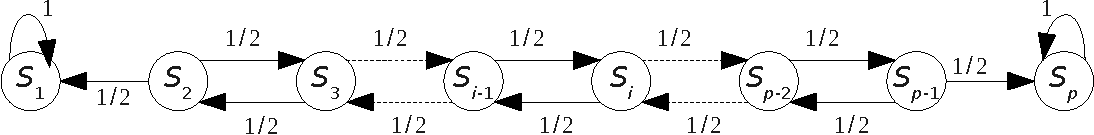
\includegraphics[width=\textwidth]{FIGS/drunk_mans_walk_absorbing}
}

\frame{\frametitle{The transition matrix for DMW 2.0}
\[
P=\begin{pmatrix}
1 & 0 & 0 & 0 & 0 & \cdots & 0\\
1/2 & 0 & 1/2 & 0 & & & \\
0 & 1/2 & 0 & 1/2 & & & \\
\vdots & & \ddots & \ddots & \ddots & & \vdots \\
& & & & & & \\
& & & & 1/2 & 0 & 1/2 \\
& & & & 0 & 0 & 1
\end{pmatrix}
\]
}

\frame{\frametitle{Put $P$ in standard form}
Absorbing states are $S_1$ and $S_p$, write them first, then write other states.
\begin{center}
\begin{tabular}{c|cccccccc}
 & $S_1$ & $S_p$ & $S_2$ & $S_3$ & $S_4$ & $\cdots$ & $S_{p-2}$ & $S_{p-1}$ \\
\hline
$S_1$ & 1 & 0 & 0 & 0 & 0 & $\cdots$ & 0 & 0 \\
$S_p$ & 0 & 1 & 0 & 0 & 0 & $\cdots$ & 0 & 0 \\
$S_2$ & 1/2 & 0 & 0 & 1/2 & 0 & $\cdots$ & 0 & 0 \\
$S_3$ & 0 & 0 & 1/2 & 0 & 1/2 & $\cdots$ & 0 & 0 \\
$\vdots$ &  &  &  &  & & & & \\
$S_{p-2}$ & 0 & 0 & 0 & 0 & 0 & $\cdots$ & 0 & 1/2 \\
$S_{p-1}$ & 0 & 1/2 & 0 & 0 & 0 & $\cdots$ & 1/2 & 0
\end{tabular}
\end{center}
So we find
\[
P=\begin{pmatrix}
\mathbb{I}_2 & \mathbf{0} \\
R & Q
\end{pmatrix}
\]
where $\mathbf{0}$ a $2\times(p-2)$-matrix, $R$ a $(p-2)\times 2$ matrix and $Q$ a $(p-2)\times (p-2)$ matrix
}

\frame{
\[
R=
\begin{pmatrix}
1/2 & 0 \\
0 & 0 \\
\vdots & \vdots \\
0 & 0 \\
0 & 1/2   
\end{pmatrix}
\]
and
\[
Q=
\begin{pmatrix}
0 & 1/2 & 0 & \\
1/2 & 0 & 1/2 & \\
0 & 1/2 & 0 & \\
&& \ddots & \ddots & \ddots \\
&&&& \\
0 &&& 1/2 & 0 & 1/2 \\
0 &&&&1/2 & 0
\end{pmatrix}
\]
}

\frame{
\[
\II_{p-2}-Q=
\begin{pmatrix}
1 & -1/2 & 0 & \\
-1/2 & 1 & -1/2 & \\
0 & -1/2 & 1 & \\
&& \ddots & \ddots & \ddots \\
&&&& \\
0 &&& -1/2 & 1 & -1/2 \\
0 &&&& -1/2 & 1
\end{pmatrix}
\]
This is a \emph{tridiagonal symmetric Toeplitz} matrix
}

\frame{\frametitle{Inverting a symmetric tridiagonal matrix}
We want to use the following result (found for example in some slides of G\'erard Meurant about Tridiagonal matrices): if 
\[
J_k=
\begin{pmatrix}
\alpha_1 & \beta_1 \\
\beta_1 & \alpha_2 & \beta_2 \\
& \ddots &\ddots &\ddots \\
&& \beta_{k-2} & \alpha_{k-1} & \beta_{k-1} \\
&&& \beta_{k-1} & \alpha_k
\end{pmatrix}
\]
\[
\delta_1=\alpha_1,\quad \delta_j=\alpha_j-\frac{\beta_{j-1}^2}{\delta_{j-1}},j=2,\ldots,k
\]
\[
d^{(k)}_k=\alpha_k,\quad d^{(k)}_j=\alpha_j-\frac{\beta_j^2}{d^{(k)}_{j+1}},j=k-1,\ldots,1
\]
then we have the result on the next slide
}

\frame{\frametitle{Inverse of a symmetric tridiagonal Toeplitz matrix}
\begin{theorem}
The inverse of the symmetric tridiagonal Toeplitz matrix $J_k$ is given by
\[
(J_k^{-1})_{ij} = (-1)^{j-i}\beta_i\cdots\beta_{j-1}\frac{d_{j+1}^{(k)}\cdots d_k^{(k)}}{\delta_i\cdots\delta_k},\;\forall i,\forall j>i
\]
\[
(J_k^{-1})_{ii} = \frac{d_{i+1}^{(k)}\cdots d_k^{(k)}}{\delta_i\cdots\delta_k},\;\forall i
\]
\end{theorem}
}

\frame{
Note that $\alpha_1=\cdots=\alpha_k=1$ and $\beta_1=\cdots=\beta_{k-1}=-1/2$. Write $\alpha:=\alpha_i=1$ and $\beta:=\beta_i=-1/2$. We have $\delta_1 = \alpha = 1$, and the general term takes the form
\[
\delta_j = \alpha-\frac{\beta^2}{\delta_{j-1}}=1-\frac{1}{4\delta_{j-1}},\quad j=2,\ldots,k
\]
\begin{align*}
\delta_2 &= 1-\frac 14= \frac 34 \\
\delta_3 &= 1-\frac{1}{4\frac 34} = \frac 23 \\
\delta_4 &= 1-\frac{1}{4\frac 23} = 1-\frac 38 = \frac 58 \\
\delta_5 &= 1-\frac{1}{4\frac 58} = 1-\frac 25 = \frac 35 \\
\delta_6 &= 1-\frac{1}{4\frac 35} = 1-\frac 5{12} = \frac 7{12} \\
\delta_7 &= 1-\frac{1}{4\frac 7{12}} = 1-\frac 37 = \frac 47
\end{align*}
}

\frame{
Taking a look at the few terms in the sequence, we get the feeling that
\[
\delta_{2n}=\frac{2n+1}{4n} \textrm{ and } \delta_{2n+1}=\frac{n+1}{2n+1}
\]
A little induction should confirm this. Induction hypothesis (changing indices for odd $\delta$):
\[
\mathcal{P}_n:
\begin{cases}
\delta_{2n-1} &= \frac{n}{2n-1} \\
\delta_{2n} &= \frac{2n+1}{4n}
\end{cases}
\]
$\mathcal{P}_1$ is true. Assume $\mathcal{P}_j$. Then
\[
\delta_{2j+1} = 1-\frac{1}{4\delta_{2j}}=1-\frac{1}{4\frac{2j+1}{4j}}=1-\frac{j}{2j+1}=\frac{j+1}{2j+1}
\]
\[
\delta_{2j+2} = 1-\frac{1}{4\delta_{2j+1}} = 1-\frac{1}{4\frac{j+1}{2j+1}}=1-\frac{2j+1}{4(j+1)}=\frac{2(j+1)+1}{4(j+1)}
\]
So $\mathcal{P}_{j+1}$ holds true
}

\frame{
In fact, we can go further, by expressing
\[
\delta_{2n}=\frac{2n+1}{4n} \textrm{ and } \delta_{2n+1}=\frac{n+1}{2n+1}
\]
in terms of odd and even $j$. If $j$ is even,
\[
\delta_j=\frac{j+1}{2j}
\]
while if $j$ is odd,
\[
\delta_j=\frac{(j+1)/2}{j}
\]
But the latter gives
\[
\delta_j=\frac{j+1}{2j}
\]
so this formula holds for all $j$'s
}

\frame{
For the $d_j^{(k)}$'s, we have $d_k^{(k)}=1$ and
\[
d_j^{(k)} = 1-\frac{1}{4d_{j+1}^{(k)}}
\]
So $d_k^{(k)}=\delta_1$ and
\[
d_{k-j+1}^{(k)} = \delta_j=\frac{j+1}{2j},\quad j=2,\ldots,k
\]
The form
\[
d_j^{(k)} = \delta_{k-j+1}
\]
will also be useful. In summary,
\begin{center}
\begin{tabular}{c|c|c|c|c|c|c}
$\delta_1$ & $\delta_2$ & $\cdots$ & $\delta_j$ & $\cdots$ & $\delta_{k-1}$ & $\delta_k$ \\
\hline
$d_k^{(k)}$ & $d_{k-1}^{(k)}$ & $\cdots$ & $d_{k-j+1}^{(k)}$ & $\cdots$ & $d_2^{(k)}$ & $d_1^{(k)}$ \\
\hline
1 & $\frac 34$ & $\cdots$ & $\frac{j+1}{2j}$ & $\cdots$ & $\frac{k}{2(k-1)}$ & $\frac{k+1}{2k}$
\end{tabular}
\end{center}
}

\frame{
In $J^{-1}$, the following terms appear
\[
\frac{d_{j+1}^{(k)}\cdots d_k^{(k)}}{\delta_i\cdots\delta_k},\;\forall i,\forall j>i
\]
and
\[
\frac{d_{i+1}^{(k)}\cdots d_k^{(k)}}{\delta_i\cdots\delta_k},\;\forall i
\]
}

\frame{
We have, $\forall i$,
\begin{align*}
\frac{d_{i+1}^{(k)}\cdots d_k^{(k)}}{\delta_i\cdots\delta_k}
&= \frac{\delta_{k-(i+1)+1}\cdots\delta_{k-k+1}}{\delta_i\cdots\delta_k} \\
&= \frac{\delta_{k-i}\cdots\delta_{1}}{\delta_i\cdots\delta_k} \\
&= \frac{\delta_{1}\cdots\delta_{k-i}}{\delta_i\cdots\delta_k} \\
&= \frac{\prod\limits_{j=1}^{k-i}\frac{j+1}{2j}}{\prod\limits_{j=i}^{k}\frac{j+1}{2j}} \\
&= \prod\limits_{j=1}^{k-i}\frac{j+1}{2j}\prod\limits_{j=i}^{k}\frac{2j}{j+1}
\end{align*}

}

\end{document}
